%! Author = Bernát
%! Date = 2025. 10. 29.
% LaTeX mintafájl szakdolgozat és diplomamunkáknak az
% SZTE Informatikai Tanszekcsoportja által megkövetelt
% formai követelményeinek megvalósításához
% Modositva: 2011.04.28 Nemeth L. Zoltan
% A fájl használatához szükséges a magyar.ldf 2005/05/12 v1.5-ös vagy késõbbi verziója
% ez letölthetõ a http://www.math.bme.hu/latex/ weblapról, a magyar nyelvû szedéshez
% Hasznos információk, linekek, LaTeX leirasok a www.latex.lap.hu weboldalon vannak.
%


\documentclass[12pt]{report}

%Magyar nyelvi támogatás (Babel 3.7 vagy késõbbi kell!)
\usepackage[utf8]{inputenc}
\usepackage{t1enc}
\usepackage[magyar]{babel}
% A formai kovetelmenyekben megkövetelt Times betûtípus hasznalata:
\usepackage{times}

%Az AMS csomagjai
\usepackage{amsmath}
\usepackage{amssymb}
\usepackage{amsthm}

%A fejléc láblécek kialakításához:
\usepackage{fancyhdr}

%Természetesen további csomagok is használhatók,
%például ábrák beillesztéséhez a graphix és a psfrag,
%ha nincs rájuk szükség természetesen kihagyhatók.
\usepackage{graphicx}


% saját csomagok
\usepackage{hyperref}
% Referencing
\usepackage[
backend=biber,
style=numeric,
sorting=none
]{biblatex}
\usepackage{booktabs}
\usepackage{makecell}
\usepackage{pgfplots}
\usepackage{tikz}
\pgfplotsset{compat=1.18}
\usepackage{indentfirst} % Az első bekezdés legyen behúzott
\setlength{\parindent}{1cm} % Behúzás mértéke (1 cm)
\usepackage{float}
\usepackage{listings}
\usepackage{psfrag}
\usepackage{csquotes}
\usepackage{biblatex}

\addbibresource{references.bib}

%Margók:
\hoffset -1in
\voffset -1in
\oddsidemargin 35mm
\textwidth 150mm
\topmargin 15mm
\headheight 10mm
\headsep 5mm
\textheight 237mm



% Document
\begin{document}

%A FEJEZETEK KEZDÕOLDALAINAK FEJ ES LÁBLÉCE:
%a plain oldalstílust kell átdefiniálni, hogy ott ne legyen fejléc:
\fancypagestyle{plain}{%
%ez mindent töröl:
\fancyhf{}
% a láblécbe jobboldalra kerüljön az oldalszám:
\fancyfoot[R]{\thepage}
%elválasztó vonal sem kell:
\renewcommand{\headrulewidth}{0pt}
}

%A TÖBBI OLDAL FEJ ÉS LÁBLÉCE:
\pagestyle{fancy}
\fancyhf{}
\fancyhead[L]{A nagy nyelvi modellek szemantikus képességeinek konzisztenciájának vizsgálata}
\fancyfoot[R]{\thepage}


%A címoldalra se fej- se lábléc nem kell:
\thispagestyle{empty}

\begin{center}
\vspace*{1cm}
{\Large\bf Szegedi Tudományegyetem}

\vspace{0.5cm}

{\Large\bf Informatikai Intézet}

\vspace*{3.8cm}


{\LARGE\bf A nagy nyelvi modellek szemantikus képességeinek konzisztenciájának vizsgálata}

{\LARGE\bf Analyzing the Consistency of Semantical Capabilities of Large Language Models}

\vspace*{3.6cm}


{\Large Szakdolgozat}

\vspace*{4cm}

%Értelemszerûen megváltoztatandó:
{\large
\begin{tabular}{c@{\hspace{4cm}}c}
\emph{Készítette:}     &\emph{Témavezetõ:}\\
\bf{Fábián Bernát}  &\bf{Dr. Berend Gábor}\\
informatika szakos     &egyetemi docens\\
hallgató&
\end{tabular}
}

\vspace*{2cm}

{\Large
Szeged
\\
\vspace{2mm}
2026
}
\end{center}


%A tartalomjegyzék:
\tableofcontents

%A \chapter* parancs nem ad a fejezetnek sorszámot
\chapter*{Feladatkiírás}
%A tartalomjegyzékben mégis szerepeltetni kell, mint szakasz(section) szerepeljen:
\addcontentsline{toc}{section}{Feladatkiírás}


A hallgató feladata egy olyan keretrendszer megvalósítása, amely lehetővé teszi a nagy nyelvi modellek szemantikával kapcsolatos képességeinek konzisztenciájának vizsgálatát. A kiértékelés során azt vizsgálja a keretrendszer, hogy a nagy nyelvi modellek válaszai milyen érzékenységet mutatnak olyan invarianciákra, amelyek az emberi válaszadásra nincsenek befolyással. A kísérletek során a nagy nyelvi modellek azzal kapcsolatos érzékenységének vizsgálata a cél, hogy mennyiben érzékenyek a nagy nyelvi modellek a Word-in-Context nevű feladat megoldása során az egyes inputokban szereplő mondatpárosok sorrendjének megcserélésére.

\chapter*{Tartalmi összefoglaló}
\addcontentsline{toc}{section}{Tartalmi összefoglaló}
\subsubsection{\textit{A téma megnevezése}}
    A nagy nyelvi modellek szemantikus
képességeinek konzisztenciájának vizsgálata.


\subsubsection{\textit{A feladat megfogalmazása}}
    A vizsgálathoz használandó adathalmaz a \href{https://pilehvar.github.io/wic/}{Word-in-Context dataset}. A kérdéseket egyenes és fordított sorrendben is fel kell tenni a modelleknek, majd összehasonlítani a válaszaikat az azonos tartalmú, de felcserélt szósorrendű kérdésekre, ezzel felmérve a szemantikus képességeiket és nyelvi konzisztenciájukat erre az emberek számára triviális, de a modellek számára problémát okozó feladat megoldására.

 \subsubsection{\textit{A megoldási mód}}
    % Ez lényegében egy optimalizálási feladat, az optimalizálandó paraméterek a modellnek beadott prompt és a választott modell.
    Akkor tekintjük helyesnek a megoldást, ha a program futtatására a kiválasztott modell egyértelmű igen/nem válaszokat ad az eldöntendő kérdésekre. A válaszainak helyessége viszont másodlagos, de nem elhanyagolható. A nyelvi modellek a Hugging Face platformról lesznek választva.

    A program bemenete tetszőleges sornyi bejegyzés a Word-in-Context adathalmaz 'test' splitjéből (vagy tetszőleges, ezzel megegyező formátumú kérdéshalmaz) és tetszőleges modell a Hugging Face platformról.

    A megoldás kulcsa olyan szoftver fejlesztése, amely mindezt minél egyszerűbbé, automatizáltabbá és gördülékenyebbé teszi.
    %         \item Összehasonlító teljesítményvizsgálatot végeztem a
    %         % TODO update-elni Gemma3-ra és QWEN3-ra mindenhol
    %         \href{https://huggingface.co/microsoft/Phi-4-mini-instruct}{Phi-4-mini-instruct}, \href{https://huggingface.co/google/gemma-2-2b-it}{Gemma-2-2b-it} és a \href{https://huggingface.co/Qwen/Qwen1.5-1.8B-Chat}{Qwen1.5-1.8B-Chat} között egy Google Colab szkriptben.
    %     \item
    %           Saját adatfeldolgozó kiértékelő Python modult készítettem a promptolás automatizálásához és a modell válaszok feldolgozására.


      % \end{itemize}
 \subsubsection{\textit{Az alkalmazott eszközök, módszerek}}

        Alkalmazott eszközök:
      \begin{itemize}
        \item Google Colab és PyCharm, Python futtatókörnyezet
        \item Git, GitHub
        \item Hugging Face
        \item A torch, transformers, accelerate és számos egyéb Python könyvtár a Hugging Face modellek használatához
      \end{itemize},

        Alkalmazott módszerek:
      \begin{itemize}
        \item Objektumorientált programozás
        \item Clean Code alapelvek \textit{Martin és Robert Clean Code} c. könyve \cite{martin2008cleancode} alapján
      \end{itemize}

  \subsubsection{\textit{Elért eredmények}}

  Elkészült a keretrendszer, egy Python konzolos program, amely képes tetszőleges Hugging Face modell válaszra bírását automatizálni. Egy kattintással vagy terminál paranccsal képes lefuttatni a  modellt az inputként megadott adathalmazra és elvégezni a nyelvi konzisztencia tesztet, statisztikákat készítve az eredményekből.

 \subsubsection{\textit{Kulcsszavak}}

       Nagy nyelvi modell, Word-in-Context, nyelvi konzisztencia, teljesítmény-összehasonlítás

\chapter*{Motiváció}
\addcontentsline{toc}{section}{Motiváció}

Az informatika és a nyelvtechnológia fejlődésével a generatív mesterséges intelligencia mindennapjaink részévé vált. A nagy nyelvi modellek kiértékelésére számos teljesítményteszt (benchmark) fejlődött ki az évek során. Az egyik legnépszerűbb ilyen teljesítményteszt a SuperGLUE Benchmark, amely 8 komoly kihívást jelentő feladat elé
állítja a nagy nyelvi modelleket. A WiC (Word-in-Context) probléma a SuperGlue 8 feladatának egyike. Az emberi
szöveget értő nyelvi modellek fejlesztése kiemelten fontos mind az akadémiai kutatásban, mind a gyakorlati alkalmazásokban. Az angol nyelvű szövegek feldolgozása nem csak az angolszász területeken releváns, hanem Magyarországon is, hiszen az angol nyelv használata a számítógépek világában mindennapjaink része. Az egyetem és a helyi vállalatok is aktívan foglalkoznak természetesnyelv-feldolgozási (NLP) megoldásokkal. Az AI megoldások - Hugging Face nyelvi modellek használatának - ismerete előnyt jelent mind a munkahelyeken, mind a magánéletben. IT területen Különösen nagy előnyt jelent az AI megfelelő használatának ismerete, például a munkafolyamatok automatizálásában. Egy hatékony szoftver, amely képes Hugging Face modelleket futtatni, tehát nemcsak tudományos értékkel bír, hanem gyakorlati alkalmazásokban is közvetlen hasznot hozhat, főleg a nyelvészeti informatikai területen dolgozók számára.


\chapter{Elméleti háttér}

\section{Megelőző lépések}
A szoftver lefejlesztése előtt átelemeztem az jelenlegi legjobb módszereket és nyílt forráskódú nyelvi modelleket a Témavezetőm által javasolt LMArena és Hugging Face felületein, továbbá az utóbbiak futtatásának dokumentációját tanulmányoztam, mert azokra a szoftver elkészítéséhez szükség volt.

 \section{A szoftver}
 A megoldásom során törekedtem arra, hogy az bárki által reprodukálható legyen, ezért ingyenesen elérhető és nyílt forráskódú eszközöket (Python, GitHub, Hugging Face) használtam.

  \section{A többértelműség problémája a természetes nyelvekben}

A természetes nyelvekben a programozási nyelvekkel ellentétben egy szónak több, egymástól teljesen elkülönülő jelentése is lehet. Például az "egér" szó jelenthet egy számítógépes perifériát vagy egy állatot, és a helyes értelmezéshez a környező szavakat ismerni kell. Az ilyen jellegű többértelműségek automatikus feloldása az egyik központi problémája a természetes nyelvi rendszerek fejlesztésének.


\section{A Word in context feladat}

 A Word in context feladatot 2019-ben fogalmazta meg Mohammad Tahmed Pilehvar, abból a célból, hogy különböző transzformer és szóbeágyazasos modelleket vizsgáljanak a feladat által megfogalmazott teljesítményteszten. A WiC feladat lényege, hogy egy adott szó két különböző mondatbeli előfordulásáról eldöntse, hogy azonos értelemben szerepel-e. A természetes nyelvi feldolgozásban. Az ezt a feladatot megfogalmazó adathalmazt alkalmasnak találtuk a témavezetőmmel az általa megfogalmazott teljesítményteszt, a nagy nyelvi modellek szemantikus képességeinek konzisztenciájának vizsgálata elvégzéséhez. A kérdések már eleve csoportosítva vannak azonos és különböző jelentésű mondatpárokként.

 \subsubsection{A Word in context háttere}
 A WiC csapata alapvetően a folyamatosan fejlődő modelleknek igyekezett egy nehezebb, korszerű teljesítménytesztet állítani. Míg korábban a statikus szóbeágyazások, mint például a Word2vec és a GloVe voltak elterjedtek a szójelentés feloldására, ma már elavult módszereknek számítanak. Ezek a statikus szóbeágyazások tervezésükből adódóan nem képesek modellezni a szavak szemantikájának dinamikus természetét, vagyis azt a tulajdonságot, hogy a szavak potenciálisan különböző jelentéseknek felelhetnek meg. Egy szóhoz mindig ugyanazt a szóvektort rendelik, kontextustól függetlenül. A kontextualizált szóbeágyazások kísérletet tesznek ennek a korlátnak a feloldására azáltal, hogy dinamikus reprezentációkat számítanak ki a szavakhoz, amelyek a szövegkörnyezet alapján képesek alkalmazkodni. Ilyen szóbeágyazás transzformer például a BERT, ám ennek is megvannak a korlátai. A mai igazán modern megoldások viszont már mély tanulást és jellemzően neurális hálókat használnak a modellek szójelentés-értelmező képességeinek fejlesztésére.


\section{Egy rendszer feladata a WiC adathalmazon}
Amikor valaki kiértékelő rendszert fejleszt a WiC benchmarkra, annak feladata a szavak szándékozott jelentésének azonosítása. A WiC egy bináris osztályozási feladatként van megfogalmazva. Adott egy többjelentésű szó, amely mindkét mondatban előfordul, továbbá egy szófaj címke, kettő index és két szövegrészlet. Egy rendszer feladata, hogy meghatározza, hogy a szó ugyanabban a jelentésben használatos-e mindkét mondatban. A $w$ célszó minden esetben csak egy ige vagy főnév lehet. A célszóhoz két eltérő szövegkörnyezet tartozik. Ezen szövegkörnyezetek mindegyike a $w$ egy specifikus jelentését váltja ki. A feladat annak megállapítása, hogy a $w$ előfordulásai a két szövegkörnyezetben ugyanannak a jelentésnek felelnek-e meg, vagy sem. Tehát a célszó ugyanazt a jelentést hordozza-e két különböző szövegkörnyezetben, vagy eltérőt. Ez egy összetett NLP probléma, mivel ötvözi a szójelentés-egyértelműsítés (Word Sense Disambiguation, WSD) és a kontextuális beágyazások elemeit, így a szójelentés-egyértelműsítés végrehajtásaként is értelmezhető.

\section{Az én céljaim ehhez képest}
A kutatásom első felének célja a modellek teljesítményének összehasonlítása a WiC-ből szedett kérdéseken volt, ám a többi rendszerrel ellentétben itt nem az volt a cél, hogy minél több kérdésre a gold standard \footnote{A gold standard egy szakértők által hitelesen és konzisztensen annotált adathalmaz, amely viszonyítási alapként szolgál automatikus rendszerek teljesítményének kiértékeléséhez.} szerint válaszoljanak, hanem hogy megvizsgáljam, hogy a nagy nyelvi modellek válaszai milyen érzékenységet mutatnak olyan invarianciákra, amelyek az emberi válaszadásra nincsenek befolyással. Ez alapján a kérdésben a mondatok sorrendje nem szabadna, hogy befolyásolja a válaszadásukat, ám azt mégis befolyásolja. Egész pontosan a
\begin{verbatim}
Does the word `w` mean the same thing in `s1` and `s2`?
\end{verbatim}
és a
\begin{verbatim}
Does the word `w` mean the same thing in `s2` and `s1`?
\end{verbatim}

kérdésekre mindig ugyanazt kellene, hogy válaszolják (változatlan $w$, $s1$ és $s2$ esetén, ahol $w$ egy szó, $s1$ az első példamondat, és $s2$ a második példamondat).

\section{Bináris osztályozás}
A WiC feladat egy bináris osztályozási (binary classification) problémaként van megfogalmazva: el kell dönteni, hogy egy adott szó két különböző mondatbeli előfordulása ugyanabban az értelemben szerepel-e.
A bináris osztályozási feladatok problémakörében is változnak a trendek olyan szempontból, hogy egyre inkább a neurális hálók és nagy nyelvi modellek az elterjedtek bináris osztályozási feladatokra is. A Lesk-algoritmus~\cite{lesk1986automatic} egy klasszikus szóértelem-felismerő módszer, amely a szótári definíciók és a kontextus összevetésével próbálja meghatározni a szó legmegfelelőbb jelentését. A legjobbak mégis az olyan, kifejezetten emberi szöveg megértésére specializálódott nagy nyelvi modellek, mint például a GPT-4.5 és a Gemini-2.5 - 2025 végén.

\label{wic:dataset}
\section{A WiC adathalmaz eredete}

A \href{https://pilehvar.github.io/wic/}{Word in Context adathalmaz} egy jó minőségű, nyelvészeti szakértők által készített benchmark adathalmaz. A mondatok a WordNetből, a VerbNetből és a Wikiszótárból származnak.
A WiC adathalmaz segítségével megvizsgálhatjuk, hogy egy rendszer (modell, algoritmus) mennyire képes a szavak jelentését megérteni különböző kontextusokban. A WiC feladat része a SuperGlue~\cite{sarlin2020superglue} Benchmarknak, amely egy széles körben elfogadott benchmark nyelvi modellek kiértékelésére. 8 feladatból áll:
\begin{itemize}
	\item  BoolQ (Boolean Questions)
	\item  CB (CommitmentBank)
	\item COPA(Choice of Plausible Alternatives)
	\item MultiRC (Multi-Sentence Reading Comprehension)
	\item ReCoRD(Reading Comprehension with Commonsense Reasoning Dataset)
	\item RTE(Recognizing Textual Entailment)
	\item \textbf{WiC(Word-in-Context)}
	\item  WSC (Winograd Schema Challenge)
\end{itemize}

A SuperGLUE a GLUE továbbfejlesztett változata, amelyet 2019-ben vezettek be, mivel a GLUE feladatait a legmodernebb modellek (pl. BERT) már túl jól megoldották. ~\cite{wang2020superglue}
Ez az egyik legszélesebb körben elfogadott benchmark, amelyen számos nyelvi modell teljesítményét vizsgálták.
A WiC halmaz fel van osztva tanító, validációs és teszthalmazra, ezért gépi tanításra egyszerűen felhasználható. Ezt segíti elő az is, hogy az összes mondat tokenekre bontott, tabulált és egységesek az írásjelek is.
A modelleket hasonlóan tanítják, mint ahogy az iskolában tanulnak a diákok.
A benchmarkok feladatait jellemzően 3 részre vágják:
tanító, validációs és teszthalmazra. Ennek az aránya eltérő lehet, de a tanítónak jóval nagyobbnak kell lennie, mint a másik kettőnek, és a teszthalmaznak nagyobbnak kell lennie, mint a validációs halmaznak. 80-10-10\%-os eloszlás a standard, ezzel, vagy hasonló eredménnyel érhetőek általában el a legjobb eredmények.

A tanító adatbázist a korábbi iskolai példára visszatérve úgy képzelhetjük el, hogy ez a leadott anyag. A validációs halmaz olyan, mint egy mintavizsga, minta ZH. A teszthalmaz pedig a végső megmérettetés, a vizsga. Fontos, hogy a teszthalmazon sose tanítsuk a modelleket, és sose legyen átfedés a halmazok között. Ez ugyanis magoláshoz vezet, és a modell nem lesz képes általánosítani.

\begin{table}[H]
    \centering
    \caption{A WiC adathalmaz tesztkészletének néhány bejegyzése}
    \label{tbl:wic_peldak} % Egyedi címke a táblázathoz
    \begin{tabular}{llcp{0.33\textwidth}p{0.33\textwidth}} % Oszlopdefiníciók: l=balra, c=középre, p{szélesség}=paragrafus adott szélességgel
        \hline
        \textbf{Szó} & \textbf{Szófaj} & \textbf{Index} & \textbf{1. Példamondat} & \textbf{2. Példamondat} \\
        \hline
        defeat      & N      & 4-4       & It was a narrow defeat.                             & The army's only defeat.                                             \\
        groom       & V      & 0-1       & Groom the dogs.                                     & Sheila groomed the horse.                                            \\
        penetration & N      & 1-1       & The penetration of upper management by women.       & Any penetration, however slight, is sufficient to complete the offense. \\
        hit         & V      & 1-3       & We hit Detroit at one in the morning but kept driving through the night. & An interesting idea hit her.                                         \\
        \hline
    \end{tabular}
\end{table}

\subsection{Korábbi eredmények a WiC adathalmazon}
A \href{https://pilehvar.github.io/wic/}{Word-in-Context honlapján} található egy eredménytábla, amely bemutatja, hogy egyes modellek és algoritmusok milyen eredményt értek el a WiC feladatra. WiC adathalmazon számos modellt teszteltek, amelyek túlnyomórészt 60\% feletti eredménnyel kategorizálták helyesen a mondatokat.
A legjobb eredményt a SenseBERT-large rendszerrel érték el, külső erőforrások használatával. Ez az eredmény megközelíti a kézi, emberi szintű kiértékelést, melynek a felső határa 80\% körüli. A kézi kiértékelésnek és a SenseBERT megoldásának egyszerűsített változatát én is elvégeztem. A kézi kiértékelésemmal közel 65, míg a Python algoritmusommal is közel 60\%-os pontosságot sikerült elérnem.


% Requires: \usepackage{booktabs}
\begin{table}[h]
    \centering
    \begin{tabular}{l l c}
        \toprule
        \textbf{Kategória} & \textbf{Implementáció} & \textbf{Pontosság \%} \\
        \midrule
        \multicolumn{3}{l}{\textbf{Sentence-level contextualised embeddings}} \\
        SenseBERT-large\textsuperscript{†} & Levine et al (2019) & 72.1 \\
        KnowBERT-W+W\textsuperscript{†} & Peters et al (2019) & 70.9 \\
        RoBERTa & Liu et al (2019) & 69.9 \\
        BERT-large & Wang et al (2019) & 69.7 \\
        Ensemble & Gari Soler et al (2019) & 66.7 \\
        ELMo-weighted & Ansell et al (2019) & 61.2 \\
        \midrule
        \multicolumn{3}{l}{\textbf{Word-level contextualised embeddings}} \\
        WSDT\textsuperscript{†} & Loureiro and Jorge (2019) & 67.7 \\
        BERT-large & WiC's paper & 65.5 \\
        Context2vec & WiC's paper & 59.3 \\
        Elmo & WiC's paper & 57.7 \\
        \midrule
        \multicolumn{3}{l}{\textbf{Sense representations}} \\
        LessLex & Colla et al (2020) & 59.2 \\
        DeConf & WiC's paper & 58.7 \\
        S2W2 & WiC's paper & 58.1 \\
        JBT & WiC's paper & 53.6 \\
        \midrule
        \multicolumn{3}{l}{\textbf{Sentence level baselines}} \\
        Sentence Bag-of-words & WiC's paper & 58.7 \\
        Sentence LSTM & WiC's paper & 53.1 \\
        \midrule
        \multicolumn{3}{l}{\textbf{Random baseline (véletlenszerű kiértékelés)}} \\
        & 50.0 \\
        % TODO kiegészíteni a saját eredményemmel
        % \midrule
        % \multicolumn{3}{l}{\textbf{Fábián Bernát kézi kiértékelés}} \\
        % & xx.x
        % \multicolumn{3}{l}{\textbf{Saját PyCharmos implementáció kiértékelés}} \\
        % & 60.x
        \bottomrule
    \end{tabular}
    	\caption{Forrás: \href{https://pilehvar.github.io/wic/}{The Word-in-Context Dataset}}

    \label{tab:state_of_the_art}
\end{table}


\clearpage


\section{Nagy nyelvi modellek}

A nagy nyelvi modell (angolul Large Language Model, LLM) olyan számítási modell, amely képes értelmes szöveg generálására vagy más természetes nyelvi feldolgozási feladatok elvégzésére. Ezek a modellek egy rendkívül költséges folyamat révén, hatalmas mennyiségű szöveges adat feldolgozásával és mélytanulási technikák alkalmazásával sajátítják el a nyelv megértését és előállítását. Az LLM-ek, mint például az OpenAI GPT-sorozata, a Google Gemini vagy a Meta LLaMA modelljei, különböző architektúrákat használnak, de leggyakrabban a transzformer alapú megközelítést alkalmazzák. Mint nyelvi modellek, az LLM-ek úgy sajátítják el ezeket a képességeket, hogy óriási mennyiségű szövegből, egy önfelügyelt és egy félig felügyelt tanulási folyamat során, statisztikai összefüggéseket tanulnak meg. Ezek a modellek  képesek összetett feladatok elvégzésére, mint például szövegfordítás, összefoglalás, információ-kinyerés, kérdés-válasz és kreatív szövegalkotás. Finomhangolás által specializált feladatokra. Nagy nyelvi modelleknek jellemzően az 50 milliárd paraméteresnél nagyobb modelleket hívják. Az ennél kisebb modelleket inkább csak nyelvi modelleknek hívom.

Inputként kap egy promptot, egy legfeljebb \texttt{n} token hosszúságú szöveget, ahol az \texttt{n} függ a modelltől és a paraméterezéstől. Erre fog legfeljebb \texttt{m} hosszúságú válaszban inferenciával, azaz következtetéssel válaszolni. Azért hívják modellnek a modelleket, mert az emberi nyelvet és kommunikációt utánozzák (modellezik).

Forrás: \href{https://hu.wikipedia.org/wiki/Nagy_nyelvi_modell}{Wikipédia}

\subsection{Chatbot Arena, vagy LMSYS - nagy nyelvi modelleket összehasonlító platform}
Kutatómunkám első lépéseként utánanéztem, hogy melyik modellek a legjobbak angol nyelvű instruction following feladatokban. Ehhez a \href{https://lmarena.ai/}{LMArenát}~\cite{chiang2024chatbot} megfelelő referenciának tartottam, mert ez az oldal igen lenyűgöző módon minden ismertebb ingyenes nagy nyelvi modellhez API-n keresztüli limitált hozzáférést biztosít: 2025. május 16-án 101 modell API-ja volt kipróbálható az oldalon keresztül több tucatnyi cégtől, a ranglétrán pedig 241 modell teljesítményét mérhetjük össze különböző kategóriák alapján emberi szavazatok alapján, amely több mint 1.5 millió ember szavazatán alapszik.
A folyamatosan frissülő rangsor menüben az opciók közül az "Instruction Following" és az "English" kategóriát vizsgáltam meg, mert a problémám ehhez a területhez áll a legközelebb.


Az oldalon található modellek mind elérhetőek és kipróbálhatóak, és általában saját, felhasználóbarát webes felületük is van, amely személyre szabható, elmenthetőek a korábbi beszélgetéseink, és egyéb kényelmes szolgáltatásokkal kecsegtetnek. Azonban fontos észben tartanunk, hogy ezeket a felületeket fejlesztő cégek bármilyen publikus webes forrást felhasználhatnak a modelljeik tanításához, beleértve a chatben megadott információt.
A nagy cégeknek, mint például a Google-nek, az OpenAI-nak és a DeepSeek-nek is vannak nyílt forráskódú, jó minőségű modelljeik, melyek hatalmas adathalmazokon be vannak tanítva. Például a GPT-3 tanítása során a Common Crawl Wikipédiát, WebText2 reddit posztokból és linkjeiből kinyert adatokat, internetes könyveket és az angol nyelvű wikipédiát is felhasználták.~\cite{springboard2023gpt3}

A nagy tech cégek, mint a Meta és az X, felhasználják a közösségi médiára feltöltött adatainkat a modelljeik fejlesztéséhez. A Google pedig a felhasználási feltételeit is többször megváltoztatta, hogy felhasználhassa szolgáltatásainak felhasználói adatait az AI termékei fejlesztéséhez. ~\cite{tan2024terms}


A Hugging Face~\cite{wolf2019huggingface} [\href{https://huggingface.co/models}{több mint 1.7 millió modellt}] és [\href{https://huggingface.co/datasets}{csaknem 400 ezer adathalmazt}] kínál különféle gépi tanulási feladatokra, beleértve a természetes nyelvfeldolgozást, képfeldolgozást és kódgenerálást is. Ezek a modellek nyilvánosan elérhetők és szabadon használhatók.
Előnyük, hogy nyílt forráskódúak, így tetszőlegesen módosíthatóak. Emellett biztonságosak: letölthetőek saját gépre, kódból futtathatóak anélkül, hogy egy szerverrel kommunikálnának. Emiatt érzékeny adatok feldolgozására is alkalmasak. Jellemzően minél kisebb a paraméterszámuk, annál gyengébb a visszaemlékező képességük, rövidebb válaszokat részesítenek előnyben, és annál gyakrabban követnek el hibákat vagy nyelvi torzulásokat - például nyelvtani hibákat, kódban szintaktikai hibákat, inkoherens (összefüggéstelen, logikailag következetlen) válaszokat. Előnyük viszont, hogy gyengébb hardveren is gyorsabban, kevesebb memóriát fogyasztva képesek futni. Nagyméretű modellek gyengébb hardveren való futtatására nyújt megoldást a kvantálás. A kvantálás általában csak a népszerűbb/nagyobb modelleknél (pl. Llama, Gemma, Mistral) elérhető, és gyakran közösségi kontribúciók eredménye (nem hivatalos verziók). A kvantálás a modell súlyait alacsonyabb bitmélységűre (pl. 32 → 8/4 bit) konvertálja, ami csökkenti a memóriaigényt és gyorsítja a következtetést. Emiatt azonban könnyen félrevezethetőek és könnyen hallucinálnak is. Ráadásul a korlátozott kontextusmegértés a csökkentett bitmélység miatt nehezebben követik a hosszú gondolatmeneteket és a gyenge memóriájuk.

\clearpage

\section*{Fogalmak}

\addcontentsline{toc}{section}{Nyelvi modell alapfogalmak}

Ahhoz, hogy nagy nyelvi modelleket ki tudjunk értékelni, meg kell ismernünk néhány alapfogalmat.

\subsection{A prompt}
A prompt alatt generatív mesterséges intelligenciák esetében egy nagy nyelvi modell számára beadott olyan inputot értünk, amelyre a modell egy előre meghatározott kimenetet generál. Működési elve lényegében ugyanaz, mint egy hagyományos konzolnak, parancssori interfésznek, például egy Windows rendszeren a PowerShell, vagy Linuxon Bash terminállal, azonban prompt esetén a kommunikáció emberi nyelven történik.
Egy jelentős előnye a promptolásnak, hogy nem csak egy előre meghatározott parancskészletet használhatunk, hanem bármit beírhatunk, nincsenek szintaktikai hibák vagy futtatási hibák, mivel a rendszer minden bemenetre képes választ generálni.

\subsection{Inferencia}
Egy modell promptra adott válaszát inferenciának nevezzük, ami következtetést jelent. Ez arra utal, hogy a modell a megtanult minták alapján futásidőben logikailag következtet a legvalószínűbb kimenetre, bonyolult statisztikai számítással, nem pedig csak szó szerint "visszadobva" a betanított adatokat.

\subsection{Determinisztikus következtetés, temperature, top-p és top-k}
A Google Colabban elvégzett kísérletemnek csak akkor van értelme, ha a futtatás determinisztikus. Azt jelenti, hogy a modell mindig ugyanazt a kimenetet adja ugyanazon bemenet esetén, mivel a véletlenszerűséget kizáró paraméterekkel (pl. $temperature=1.0$, $top-k=0$, $top-p=1.0$) működik. A temperature (hőmérséklet) a nyelvi modellek válaszainak kreativitását szabályozza (magas értéknél változatosabb, alacsonynál determinisztikusabb kimenet), a top-k pedig korlátozza a következő szó választékát a k legvalószínűbb tokenre, míg a top-p (más néven nucleus sampling) dinamikusan választja ki a valószínűségi eloszlás egy részhalmazát (pl. a legvalószínűbb tokeneket, amelyek összege eléri a p küszöböt)~\cite{holtzman2020curious}.

Tegyük fel, hogy a nyelvi modellnek a következő mondatot kell befejeznie:

\begin{verbatim}
The cat sat on the _ .
\end{verbatim}
A modell célja, hogy megtalálja a legmegfelelőbb szót a hiányzó helyre. Ehhez különböző mintavételi stratégiákat alkalmazhat, például a top-k vagy top-p eljárást.
A top-k módszer során a modell kiszámítja az összes lehetséges folytatás valószínűségét, majd ezek közül kiválasztja a k legvalószínűbbet, a többit pedig elveti. A kiválasztott k szóból ezt követően véletlenszerűen választ egyet, amelyet a szöveg folytatásához használ. Ez a megközelítés biztosítja, hogy csak a legrelevánsabb szavak kerüljenek figyelembe vételre, ugyanakkor némi változatosságot is megtart a generálásban.

\begin{figure}[htbp]
\centering

\vspace{0.5em}
\small\textit{A modell szerint az alábbi 5 szó a legvalószínűbb, csökkenő eséllyel: mat, hat, dog, sofa, floor.}

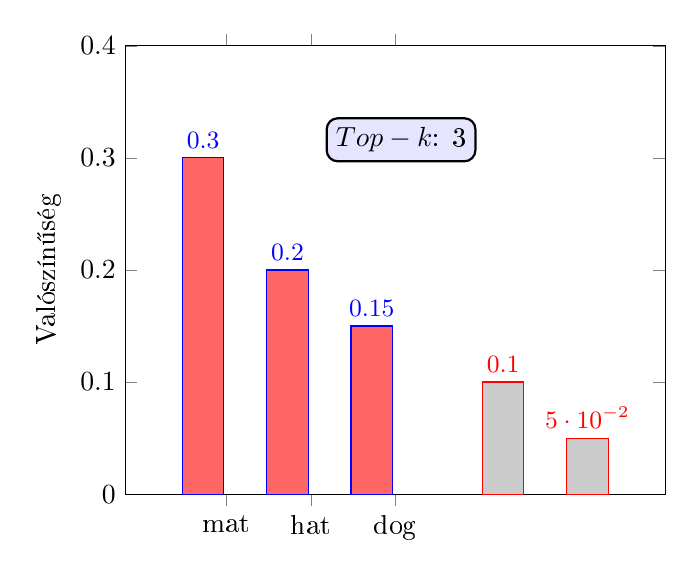
\begin{tikzpicture}
  \begin{axis}[
    ylabel={Valószínűség},
    xtick=data,
    symbolic x coords={mat, hat, dog, sofa, floor},
    ybar,
    nodes near coords style={font=\small},
    nodes near coords,
    bar width=15pt,
    enlarge x limits=0.3,
    ymin=0,
    ymax=0.4,
  ]
    % Top-3: mat, hat, dog — highlight with red fill and bold labels
    \addplot+[ybar, fill=red!60] coordinates {
      (mat,0.3) (hat,0.2) (dog,0.15)
    };
    \addplot+[ybar, fill=gray!40] coordinates {
      (sofa,0.1) (floor,0.05)
    };
  \end{axis}

  % Top-k info
  \node[draw, thick, align=center, fill=blue!10, rounded corners] at (3.5,4.5) {$Top-k$: 3};
\end{tikzpicture}

\caption{A top-k=3 értékadás esetén a pirossal kiemelt szavak közül fog diszkrét valószínűségi eljárás szerint választani.}
\end{figure}


A $top-p$ működése hasonló. Annyiban tér el, hogy nem egy fix számú legvalószínűbb szót választunk ki, hanem az odaillő szavak valószínűsége szerint. A $p$ egy 0.00-tól 1.00-ig terjedő valós szám. A szavakat akkumulatívan vesszük számításba, amíg a $p$ értéke nagyobb, mint a soron következő legvalószínűbb szó valószínűsége, addig belevesszük a szót és ugrunk előre. Ellenkező esetben csak belevesszük a szót, és leáll az algoritmus. Ezzel a módszerrel minél nagyobb a $p$ érték, annál több szó közül lehet választani, de legalább 1 szót kapunk, tehát mindenképpen tudjuk folytatni a szöveget.



\subsection{Maximum kimeneti tokenek és kontextusablak}

A \textbf{maximum kimeneti tokenek} paraméter határozza meg, hogy a modell legfeljebb hány tokent generálhat a válasz során. Ez kizárólag a válasz hosszát korlátozza, nem befolyásolja közvetlenül a bemeneti szöveget.


A \textbf{kontextusablak} (angolul \textit{context window}) a modell által egyszerre figyelembe vehető tokenek teljes száma – beleértve a bemenetet és a választ is. Ha a bemenet vagy a beszélgetés túl hosszú, a legrégebbi részek elvesznek. A GPT-4 esetében például ez elérheti a 8192 vagy akár 32\,768 tokent is, verziótól függően. ~\cite{https://community.openai.com/t/what-is-the-context-window-of-gpt-4/701256} % TODO into bib


\chapter{Legkonzisztensebb nagy nyelvi modellek megtalálása}

\subsubsection{Konzisztencia}
Mint ahogy már írtam, a kutatásom célja a modellek teljesítményének összehasonlítása a WiC-ből szedett kérdéseken volt, ám nem az volt a cél, hogy minél több kérdésre a gold standard szerint válaszoljanak, hanem hogy a szavak sorrendje ne befolyásolja a válaszadásukat. Tehát a
\begin{verbatim}
Does the word `w` mean the same thing in `s1` and `s2`?
\end{verbatim}
és a
\begin{verbatim}
Does the word `w` mean the same thing in `s2` and `s1`?
\end{verbatim}

kérdésekre mindig ugyanazt válaszolják (változatlan $w$, $s1$ és $s2$ esetén, ahol $w$ egy szó, $s1$ az első példamondat, és $s2$ a második példamondat).

Először a LMArena modelleket vizsgáltam meg, hogy mennyire érzékenyek arra, hogyha a 2 mondatot felcseréljük. A WiC adathalmazból előállított kérdésekből szúrópróbaszerűen adtam be kérdéseket a vizsgált modellnek, majd töröltem a modell memóriáját, és ezt a kérdést a 2 mondatot felcserélve is elküldtem a modellnek. A mondatokat ~\ref{chap:src/Framework} src/Framework/ModelInputPreparer modullal hoztam létre a WiC adatbázisból, erről majd később írok. Végül egy Google Táblázatban a válaszokból összesítettem az egyes promptolási módszerek pontosságát, kiegyensúlyozott pontosságát, hogy mekkora arányban egyeznek a válaszpárok. A teszthalmazban alapból randomizált sorrendben vannak a kérdések.
\begin{equation}
    \text{pontosság} = \frac{TP + TN}{TP + TN + FP + FN}
\end{equation}
\vspace*{0.5cm}

\begin{equation}
	\text{kiegyensúlyozott pontosság} = \frac{1}{2} \left( \frac{TP}{TP + FN} + \frac{TN}{TN + FP} \right)
\end{equation}
\vspace*{0.5cm}


  {\large\bf Hugging Face modellek}

Olyan modelleket választottam az összehasonlításhoz, amelyek nyílt forráskódúak, nagyjából azonos, másfél milliárd és 5 milliárd közötti paraméterszámúak, de legfeljebb 2 milliárd paraméterszám-különbség van köztük. A \href{https://colab.research.google.com/}{Google Colab} webes Python futtatókörnyezetet, Hugging Face modelleket használtam.

Először is, ahhoz, hogy egyértelmű eredményt kapjak a modell teljesítésére, ahol csak lehetett, minden véletlenszerűséget biztosító paramétert ki kellett kapcsolnom. Erre azért volt szükség, hogy ne a szerencsén múljon az, hogy a modell két válasza megegyezik, vagy eltér, hanem a modell felépítésén. A sztochasztikus faktorokkal ugyanis ugyanarra a kérdésre eltérő futtatáskor eltérő választ adhat egy modell, ami nem vezet hiteles összehasonlításhoz. A LMArena és a Google AI Studio oldalán van erre lehetőség.

Hogy ezt elérjem, a \textit{temperature} értékét 0-ra, a \textit{top-p} értékét pedig 1-re állítottam. Ezáltal a válaszok sztochasztikus változatosságát minimálisra redukáltam.


{\large\bf Egy példa kérdés:}

{\bf Egyenes sorrendben}
\begin{quote}
	\texttt{Does the word "defeat" mean the same thing in sentences "It was a narrow defeat." and "The army's only defeat."?}
\end{quote}

{\bf Fordított sorrendben}
\begin{quote}
	\texttt{Does the word "defeat" mean the same thing in sentences "The army's only defeat." and "It was a narrow defeat."?}
\end{quote}

A véletlen faktor kikapcsolása mellett az is fontos volt, hogy egyesével adjam be a kérdéseket. Amikor ugyanis egyszerre $N$ kérdéssel bombáztam a modelleket, akkor az is egy figyelembe veendő tényező volt, hogy az $N$ kérdés milyen sorrendben lett feltéve. Ráadásul a modellek, ha egyszerre túl sok kérdést kaptak, jellemzően csak 40-60 kérdésre válaszoltak, az utána lévőket teljesen ignorálták. Ezzel szemben, ha minden kérdés esetén tiszta lappal indítottam, és új, független promptként adtam be, akkor ez a hatás nem tudott bezavarni. Emiatt tisztább a kísérlet, ha a modell nem egyszerre kapja meg mind az $N$ mondatot, amiről a döntést várjuk, hanem $N$ darab olyan kérdésként, amelyekben egyenként csak pontosan egy kérdés szerepel.

Eredetileg egy, a Témavezetőm által készített és javasolt Google Colab jegyzetfüzetet~\cite{berend2025phi} fejlesztettem tovább. Ez egy egyszerű, de hatékony jegyzetfüzet, amellyel Hugging Face token birtokában tetszőleges modell válaszadásra bírható, és mindez hatékonyan automatizálható. Ám nem voltam elégedett a környezet adta korlátozásokkal, pl. session-alapú futtatókörnyezet, amely a session végével törli az adataimat, lassú csatlakozási idő a távoli hardverekhez, limitált erőforrás-hozzáférés, perzisztens adattárolási lehetőségek hiánya. Emiatt PyCharm fejlesztői környezetet használtam a keredtendszer elkészítésére, lásd később\ref{chap:src/Framework}.


\section{A megfelelő nyelvi modellek kiválasztása}
A nagy AI cégek, mint az OpenAI, Anthropic és a DeepSeek olyan fejlett általános célú generatív mesterséges intelligencia modelljeik vannak, amelyek minden kategóriában csúcsteljesítményt nyújtanak, vállvetve a Google, Microsoft, X és Meta technológiai óriásokkal, csak hogy párat említsek. Összevettettem a modelljeik webes felületén található modelljeik teljesítményét webes promptolással:


\begin{itemize}
\item \href{https://chatgpt.com}{ChatGPT} (OpenAI), amely gyors, sokoldalú, de fizetős az API-ja.
\item \href{https://claude.ai}{Claude} (Anthropic), amely biztonságközpontú, de fizetős az API-ja.
\item \href{https://chat.deepseek.com}{DeepSeek} (DeepSeek), amely hatékony, tömör, nyílt forráskódú, nagyméretű. A legnépszerűbb modell HuggingFace-en egy DeepSeek modell (a DeepSeek-R1).
\item \href{https://gemini.google.com}{Gemini} (Google)
\item \href{https://grok.x.com}{Grok} (xAI)
\end{itemize}

\begin{table}[h]
\centering
\resizebox{\textwidth}{!}{

\begin{tabular}{|l|c|c|c|}
\hline
\textbf{Modell neve} & \textbf{Helyes válaszok (db/összes)} & \textbf{Pontosság} (\%) & \textbf{Konzisztencia (\%)} \\ \hline
GPT & 143/188 & 76 & 90 \\ \hline
Claude & 138/188 & 73 & 87 \\ \hline
DeepSeek & 141/188 & 75 & 83 \\ \hline
Gemini & 156/188 & 82 & 91 \\ \hline
Grok & 126/188 & 67 & 84 \\ \hline
\end{tabular}
}
\caption{Nagy nyelvi modellek teljesítményértékelése. Az 2800 kérdés a 1400 egyenes, valamint 1400 fordított sorrendben beadott kérdésből álló prompt-korpusz egyenes és fordított beadásából tevődik össze.}
\end{table}

\section{Kiválasztott Hugging Face modellek}
A Google Colab szkriptemben~\ref{att:colab}.\\ a Témavezetőm által ajánlott modelleket, a
\begin{itemize}
    \item \href{https://huggingface.co/microsoft/Phi-4-mini-instruct}{Microsoft/Phi-4-mini-instruct}~\cite{phi4mini2024},
    \item \href{https://huggingface.co/google/gemma-2-2b-it}{Google/Gemma-2-2b-it}~\cite{gemma22b2024} és a
    \item \href{https://huggingface.co/Qwen/Qwen1.5-1.8B-Chat}{Qwen1.5-1.8B-Chat}~\cite{qwen15chat2024}
\end{itemize}
 modelleket hasonlítom össze, mert ezek elég jók méret/minőség arányban a közösségi média fórumok szerint. Közelítő arányban sincsenek a nagy AI és tech cégek top modelljeivel, de a méretükhöz képest gazdag szókinccsel és jó nyelvérzékkel rendelkeznek. Mind a hármat közepes és nehéz kérdéseken, mindkét kérdésnehézséget egyenes és fordított sorrendben teszteltem. Ez így összesen \texttt{3*3*2=18} kiértékelést jelentett. Hangsúlyozom, hogy nem a {gemma-2b-it}, hanem a {gemma-\textit{2}-2b-it} változatot választottam. Az elnevezési szabály kissé összezavaró, ugyanis {gemma-\textit{x}b...} kezdetű modellek első generációs változatok, míg a {gemma-2-\textit{x}b...} a második, és a {gemma-3-\textit{x}b...} a harmadik generációs modelleket jelöli. A gemma 3 család 2025 tavaszán tétetett közzé, így erről átfogó vizsgálatot nem végeztem, ám feltehetően jobb a szójelentés-felismerés feladatokban, mint elődje.
A modellek eredményeit összessítő táblázat a 4.1. táblázatban látható.\ref{tab:model-eval-summary}


A nagy nyelvi modelleket futtató szkriptem nyilvánosan megtekinthető, és a kísérlet elvégezhető Google Colab-on, a mellékletben található linken.~\ref{att:colab}

Mivel Google Colabot használtam, azon belül is GPU-s futtatókörnyezete, így a kiértékelés megfelelően gyors volt.
A webes környezet és a kikapcsolt valószínűségi változók miatt elmondható, hogy a kiértékelésem módja:
\begin{itemize}
	\item reprodukálható, azaz bárki meg tudja ismételni a kísérletet
	\item determinisztikus, tehát ugyanarra az inputra mindig ugyanaz lesz az output, nem függ a véletlentől.
\end{itemize}


% \section{Webes nagy nyelvi modellek}


% A modelleket fejlesztőik szerint csoportosítottam, és empirikus úton értékeltem a teljesítményüket.



% \subsection{OpenAI modellek: a GPT család}
% A GPT modellek transzformátor architektúrára épülnek, melyekben a tokenek pozíciója kulcsfontosságú. A mondatok sorrendjének felcserélése leginkább csak akkor eredményez eltérő eredményt, ha a két mondat tartalma eltérő kontextust biztosít a vizsgált szó számára. Ezek a modellek jellemzően konzisztensek a \href{https://arxiv.org/pdf/1911.00536}{többkörös, folyamatos kontextusmegőrzéses környezetekben} (amikor az inferencia során a felhasználó és a saját korábbi üzeneteit is figyelembe veszi), hiszen erre lettek optimalizálva, így nehezebben vezethetők félre.

% A \href{https://huggingface.co/docs/transformers/en/model_doc/gpt2}{gpt-2} modellt Python szkriptben is futtattam. Nem chat modell, ezért nem rendelkezik beépített chat template-tel, így a tokenizer.apply\_chat\_template() függvény hívása hibát eredményez. Ehelyett hagyományos szöveges promptot kell megadni, például egy kérdés-válasz formátumban, amit a modell egyszerűen sztringként kezel.

% \subsection{Anthropic Modellek: Claude család}

% 	      A Constitutional AI nevű saját kutatási irányon nyugszik, fókusza a biztonságos, etikus viselkedés alkotmányos szabályozással.
% 	      A Claude modellek pontos architektúrális részletei kevésbé nyilvánosak. Ezeknek a modelleknek a fő erőssége a kódolásban való kiváló segítségnyújtás, de párbeszédkonzisztencia és érvelési következtetés szempontjából kiemelkedőek. Nem jellemző, hogy a szavak és mondatok sorrendjének megváltoztatása hatására következetlen válaszokat adjon.
%           ~\cite{https://www.anthropic.com/news https://www.anthropic.com/news}


% \subsection{Microsoft Modellek: Copilot család}
% A Copilot-modellek elsősorban kódkiegészítésre optimalizáltak, így a finomabb nyelvi jelentéskülönbségekre érzékenységük alacsony. – emiatt a sorrendváltozásra adott válaszok is ingadoznak.

% \subsection{Google modellek: Gemini, Bard, Gemma}
% A Google modelljei igen előkelő helyet foglalnak el a https://lmarena.ai/ rangsorán, a Gemini-2.5-Pro-Exp-03-25 modellje az első helyet foglalja el, és a rangsor első 16 modelljéből 7 Google által fejlesztett. A gyakorlatban sokszor félreértelmezik a felhasználó szándékát, de a WiC-feladatra nagyon jól teljesítenek. A Gemma-2.5 teljes teszthalmazon 80\%-os pontosságot ért el, egyenes és fordított sorrendben is megadva.


% \subsection{Grok}
% Az xAI A Grok-3 Beta modellje erősen marketingelt, de a szójelentés átlagosnak bizonyult. A marketingkommunikáció szerint erős, de a valós teljesítménye pontatlan. A modell gyakran túlbizonyos, hibás válaszokat ad önbizalommal, és nehezen ismeri be a tévedéseit. Elon Musk nyilvános állításainak megfelelően a modell politikailag elfogult lehet bizonyos társadalmi kérdésekben. Az xAI nem tett közzé átfogó benchmark eredményeket a Grok-ról, így nehéz összehasonlítani más modellekkel. A Llama 3.2 kipróbálható Ollama telepítés után, konzolon keresztül. Hátránya a korlátozott kreativitás:  kreatív feladatokban (pl. történetírás, metaforaértelmezés) gyakran sablonos válaszokat ad.

% \subsubsection{Megjegyzés}
% Fontos megjegyeznem, hogy a modelleket csak empirikus módon véleményezem, nem végeztem átfogó kutatást. A tényleges érzékenység mértékének megállapításához alaposabb tesztekre van szükség.

% \subsection{Összegzés}
% Egy kicsit mindegyik nyelvi modell hasonlítható egy hashelő algoritmushoz abból a szempontból, hogy ha az inputot egy kis mértékben is változtatjuk, akkor az output teljesen más lehet.
% Ez akkor is igaz, ha a temperature 0-ra van állítva, magasabb temperature értékkel pedig főleg jellemző ez. Ez a viselkedés indokolt, hiszen a modellek egy jelentősebb módosítószó, pl. tagadószó, hangulatszó hatására képesek a szavak jelentésétől elrugaszkodva az eltérő kontextusra reagálni. A WiC feladatnál a mondatok fordított sorrendben való beadása ugyan nem változtat az input szemantikáján, ám a modellek sokszor tévesen más kontextusúnak gondolják azt.


\subsection{Google AI Studio}
A \href{https://aistudio.google.com/prompts/new_chat}{Google AI Studio} egy ingyenes, Google által fejlesztett platform, ahol megtalálható az összes 'state-of-the-art' modelljük, és rendkívül személyre szabhatóak. A modellek kipróbálgatása után arra a következtetésre jutottam, hogy a Gemini 2.5 Pro Experimental 03-25 a legjobb a WiC feladatra. Egy inferenciában, kevesebb mint 10 perc alatt képes válaszolni mind az 1400 tesztkérdésre, amelyekre több futtatásom esetén is közel 80\%-os pontossággal teljesített, mind egyenes, mind fordított sorrendben beadva a kérdéseket, átlagosan 91\%-os egyezéssel az egyenes és a fordított sorrendben adott válaszai alapján. Lehetségesnek tartom, hogy a sikerességéhez hozzájárul az, hogy látta a kérdéseket az előtanulítása közben, és hatékonyan vissza tudott rá emlékezni, de az mindenképpen figyelemreméltó, hogy a kézi emberi kiértékeléssel egyező hatékonyságot egyedül ez a variáns ért el.

Összességében a legkonzisztensebbek a tesztjeim alapján a Gemini-2.5 variánsai, továbbá a GPT-4 és a GPT-4.5o, ám ez csak empirikus vélemény.


\chapter{Három generatív nyelvi modell összehasonlítása Cloud környezetben}
{
	\centering % Középre igazítás a magyarázó szövegnek
	{\Large A gemma-2-2b-it, Phi-4-mini-instruct és a Qwen1.5-1.8B-Chat összehasonlítása \par} % Kisebb betűméret, sortörés

	\vspace{1cm} % Térköz a magyarázó szöveg és az első szakasz címe között
}
\section{Módszer}

\subsection{Előkészítés}
A generatív nyelvi modelleket egy Google Colab szkriptben hasonlítottam össze. Az projektem többi részét PyCharmban készítettem, ám itt a Colabra volt szükségem, mert lokálisan nagyon nehéz futtatni egy több billió paraméteres nyelvi modellt. Annál kisebbet pedig nem tartottam megfelelőnek, mert nagyon rosszul teljesítenének a WiC feladatra. Az első félévben lokálisan próbáltam futtatni "kisméretű" modelleket, azonban GPU-, RAM- és tárhelyproblémákkal küszködtem. Szerencsére a Google ingyenesen biztosít lehetőséget Cloud-alapú futtatásra, és GPU-t is biztosít. A modell egy távoli gépre töltődik le, és GPU-t is használ megfelelő beállításokkal.

\subsection{A beadott szöveg formátuma}

A modelleket úgy teszteltem, hogy eldöntendő kérdéseket tettem fel nekik egyesével:

\newenvironment{linguisticexample}
  {\par\medskip\noindent\small
   \begin{tabular}{p{0.45\textwidth}p{0.45\textwidth}}
   \textbf{Angolul} & \textbf{Magyarul} \\}
  {\end{tabular}\par\medskip}

\begin{linguisticexample}
Does the word \textit{w} mean the same thing in sentences \textit{s1} and \textit{s2}? &
Ugyanazt jelenti-e a \textit{w} szó az \textit{s1} és \textit{s2} mondatban?
\end{linguisticexample}

Ahol \textit{w} egy szó, \textit{s1} az első példamondat, és \textit{s2} a második példamondat.

% TODO delete?
\subsection{A modelleket tesztelő kérdések}
2 gondosan összeállított kérdéshalmazzal értékeltem ki a teljesítményüket.

\begin{itemize}
	\item Egyrészt a \href{https://pilehvar.github.io/wic/package/WiC\_dataset.zip}{WiC adathalmaz}ra alapuló kérdéshalmazomból szúrópróbaszerűen randomizált kérdéseket tettem fel és adtam be a modelleknek, főleg a  teszthalmazból.
    \item Másrészt, szintén a kérdéshalmazomból kiválasztottam pár hasonló szót, vagy szövegkörnyezetet tartalmazó mondatot, amelyekkel könnyű a modellt összezavarni.
\end{itemize}
A WiC megfelelő referenciaadatkészlet erre is, hiszen szakértők által gondosan annotált példákon alapul. Könnyen lehetséges, hogy már látták a tesztelt modellek (Phi, Gemma, Qwen) a WiC adathalmaz részét vagy egészét, ám nem tudnak rá visszaemlékezni, mert több milliárd mondatot láthattak a tanításuk során.

\begin{figure}[h]
\centering
% \includegraphics[width=1\linewidth]{graphics/???.png}
\caption{A mondatok természetes nyelvezetűvé alakítását végző sentence\_normalizer szkript működése.}
\label{fig:sentence-normalizer}
\end{figure}

A \href{https://pilehvar.github.io/wic/package/WiC\_dataset.zip}{WiC adathalmazban} található mondatokban a szavak, mondatjelek és írásjelek tokenizálva vannak, szóközzel vannak elválasztva a megelőző és következő szótól, mondatjeltől és írásjeltől. Így a vessző, mondatvégi pont, az angol birtokos személyjel \textquotesingle s rag és bármilyen aposztrófot használó angol rag, jel, képző könnyen kiemelhető a szövegből. Emiatt viszont külön figyelnem kellett, amikor természetes nyelvezetűvé alakítottam a szöveget, hogy ezeket is gondosan átalakítsam. Erre használtam a \texttt{sentence\_normalizer} szkriptem függvényeit~\ref{fig:sentence-normalizer}.

\vspace{6mm}
Emellett volt pár kifejezés és speciális karakter, amelyet ahhoz, hogy Python szótárként eltároljam, escape-elnem kellett, vagyis el kellett érnem, hogy a Python interpreter egyszerű karakterként kezelje őket, és ne program utasításként. A mondatokat ugyanis string dictionary-ként tároltam el, amelyekben az idézőjeleknek és kettőspont (:) karaktereknek speciális funkciója van. Így az alábbi helyzetekben gondosan átalakítottam a szöveget a Python szintaxisnak megfelelő alakba. Ezt is a \texttt{sentence\_normalizer} szkriptem függvényei végezték.

\begin{table}[h]
  \centering
  \resizebox{\textwidth}{!}{
  \begin{tabular}{|l|l|}
    \hline
    Eredeti & Átalakított \\ \hline
    \makecell[l]{My boss is out on another of his three martini lunches.\\
    Will you join us at six o'clock for martinis?} &
    \makecell[l]{My boss is out on another of his three martini lunches.\\
    Will you join us at six o\textbackslash'clock for martinis?} \\ \hline
    \makecell[l]{The derivative of f : f(x ) = x\textasciicircum 2 is f':f'(x ) = 2x.\\
    `electricity' is a derivative of `electric'.} &
    \makecell[l]{The derivative of f \: f(x ) = x\textasciicircum 2 is f\textbackslash'\:f\textbackslash'(x ) = 2x.\\
    `electricity' is a derivative of `electric\textbackslash'.} \\ \hline
  \end{tabular}
  }
  \caption{A \texttt{sentence\_normalizer} függvény átalakítása}
  \label{tab:transformed_text}
\end{table}



Én ugyanis a kutatómunkám első fázisaként a weben, távoli szerveren futó modelleken szerettem volna tesztelni, ahova a mondatok ilyen formában nem feleltek meg a kiértékelésre, mert pont az volt a célom, hogy megvizsgáljam, mennyire értik meg jól a nagy nyelvi modellek az emberi szöveget. Emiatt a listában felsorolt tokeneknek az előfordulásainál átalakítottam a szöveget: kitöröltem az előttük lévő szóközt. Ezzel lényegében visszaalakítottam a mondatokat emberi nyelvre. Ezt reguláris kifejezéseket használva és mintákat keresve Python algoritmussal oldottam meg.\ref{fig:sentence-normalizer}


\subsection{Kérdés-válasz szótár}
A naiv kérdés-válasz készítési ötlet az lehetne, hogy a vizsgált szó legyen a kulcs, és a kérdés a válasz. Ez azonban nem célszerű, sőt hibás,  ugyanis egy szóhoz több bejegyzés is tartozhat az adathalmazban, viszont a mondatpárok egyediek egymáshoz képest. Emiatt a kérdéseknek kell lenniük a kulcsoknak, amelyeknek a gold standard válasz az értéke. Például egy szótárelem kulcs-érték pár a következőképpen néz ki:
\begin{lstlisting}
Key: Does the word "w" mean the same thing in
"s1" and "s2"?
Value: Yes VAGY No
\end{lstlisting}
% end TODO delete?


\subsection{Futtatás}
A \href{https://colab.research.google.com/drive/1yA8IAd5z2oreKUXha-16Du2YrNhemNiU?usp=sharing}{Google Colab jegyzetfüzetem} esetén a modell nevének a pontos Hugging Face azonosítóját a
\begin{lstlisting}
    model_name = <company/model-name>
\end{lstlisting}
utasítással lehet megadni. Az
\begin{lstlisting}
    AutoTokenizer.from_pretrained(model_name)
\end{lstlisting}
sor létrehozza a tokenizer példányt. Ez felelős azért, hogy a nyers szöveget a modell által értelmezhető tokenekre bontsa. A \texttt{from\_pretrained} hívással automatikusan letöltöm a modellhez illő tokenizálót.
Az
\begin{lstlisting}
    AutoModelForCausalLM.from_pretrained(...)
\end{lstlisting}
függvény tölti be a nyelvi modellt, amely képes szöveget generálni. % A causal language model elnevezés arra utal, hogy a modell kategóriája szöveges következtető típus...
\begin{itemize}
	\item \texttt{device\_map='auto'} beállítás automatikusan eldönti, melyik modelltömb kerüljön melyik eszközre pl. GPU-ra vagy CPU-ra.

	    \item  \texttt{torch\_dtype='auto'} beállítás automatikusan kiválasztja a megfelelő adattípust a modellhez, pl. float16, bfloat16 adattípust.

	  \item  A  \texttt{trust\_remote\_code=True} beállítás engedélyezi a modellhez tartozó egyedi kód futtatását, abban az esetben, ha a modell nem a standard Hugging Face interfészt használja.

          \item \texttt{do\_sample=False}: Teljesen determinisztikussá teszi a futtatást. Kikapcsolja a sztochasztikus mintavételezést, és átvált mohó dekódoló üzemmódba, azaz a modell mindig a legnagyobb valószínűségű következő tokent választja ki.
\end{itemize}

A tokenizálást az \texttt{apply\_chat\_template} végzi el,
\href{https://huggingface.co/docs/transformers/main/en/chat\_templating}{amely egyesíti a különböző modellek output formátumát}.
A \texttt{Gemma} esetén a \texttt{flash-attention} csomag telepítése szükséges hozzá. Paraméterei:
\begin{lstlisting}
return_tensors='pt'        # A kimenetet PyTorch tensor formatumban kerem.
add_generation_prompt=True # Specialis jelzes, hogy generalni kell valaszt.
\end{lstlisting}

Ezután a \texttt{.to(model.device)} biztosítja, hogy az input tensor ugyanarra
az eszközre (pl. GPU) kerüljön, mint a modell.

A szöveg-generálás lépése:
\begin{lstlisting}

output = model.generate(
    inputs,
    max_new_tokens=200,     # Maximum 200 uj token
    do_sample=False,       # Determinisztikus valasz
)
\end{lstlisting}

A válasz dekódolása:
\begin{lstlisting}
decoded = tokenizer.batch_decode(output, skip_special_tokens=True)

for reply in decoded:
    print(reply)
\end{lstlisting}

\texttt{skip\_special\_tokens=True} eltávolítja az olyan vezérlő tokeneket,
mint \texttt{<s>} vagy \texttt{<|endoftext|>}, amelyek nem részei a természetes szövegnek.

Végül egy for ciklus segítségével az összes dekódolt választ szépen sorban kiírom:

\begin{lstlisting}
    for i, sentence in enumerate(decoded):
    print(f"[{i}] {sentence}")
\end{lstlisting}



A blokkot \texttt{\href{https://pytorch.org/docs/stable/generated/torch.no_grad.html}{torch.no\_grad()}} kontextusba helyeztem. Enélkül nagyon pazarolná a program a GPU memóriát, és rövid úton "out of memory" hibába futna.
A szkripttel hibátlanul le tudtam tesztelni a modelleket, amelyeket szerettem volna.

\subsection{Kiértékelés}
A nyelvi modellek hajlamosak az önismétlés hibájába esni, és az is gyakori torzulás, hogy az egyik osztályt aránytalanul preferálják a másik fölött, tehát például a WiC kérdéseinek 80\%-ára nemmel válaszolnak. A kiértékelés során figyelembe vettem, hogy ha mindegyik kérdésre ugyanazt a választ adja, és ezzel aránytalanul sokat eltalál, az ne érjen annyi pontot, mint ha közel fele-fele arányban tippel vegyesen. Más szóval, ha egy modell mindenre ugyanazt válaszolja, és történetesen ezzel jól lefedi az egyoldalú gold standardot, az nem jelent valódi tudást, csak szerencsés torzítást.
A kiegyensúlyozott pontosság (balanced accuracy) módszerével az abszolút \texttt{true positive} arány helyett egy átlagolt \texttt{true positive} arányt adunk meg az egyes osztályokra.


Ez segít, ha pl. a gold standard 80\% "Yes" és 20\% "No", de a modell mindig "Yes"-t mond – a sima pontosság 80\%, de a kiegyensúlyozott pontosség csak 50\%.

\lstset{breaklines=true}

\subsection{A modell válaszainak bővításe}
Hamar be kellett látnom, hogy az algoritmus egy puszta "Yes" vagy "No" válasza önmagában nem sok információt rejt magában. Ha csak ennyit kapok vissza, nem tudom, hogy hogyan gondolkodott a modell, milyen szóvektorai vannak.
Emiatt, hogy a puszta "Yes" és "No" válasznál többet kapjak vissza, többféle módszert alkalmaztam:
\begin{enumerate}
    \item Megkértem a modellt, hogy írja le a gondolatmenetét.
	\item A promptban utasítottam a modellt, hogy érveljen is, miért tartja helyesnek a válaszát.
        \item Megkértem, a modellt, hogy egy \textit{normalizált skálán}, mondjuk egy 0 és 100 közötti számmal, a határértékeket beleértve ítélje meg, hogy a modell mennyire biztos abban, hogy a célszó a 2 mondatban ugyanabban az értelemben van jelen. 100\% jelenti azt, hogy a modell teljesen biztos abban, hogy a célszó a 2 mondatban ugyanazt jelenti, 0\% esetén pedig teljesen biztos az ellenkezőjében.
	      \begin{lstlisting}
Answer with "Yes" or "No" with reasoning and your confidence score of "Yes" in percentage. 100% means you are a hundred percent sure that they mean the same thing, 0% means the opposite.

Does the word "{word}" mean the same thing in sentences "{sentence1}" and "{sentence2}"?
\end{lstlisting}


	      \begin{figure}[H]
	      	\centering
	      	\includegraphics[width=1\linewidth]{graphics/Answer-all-questions-with-reasoning.png}
	      	\caption{A nagy nyelvi modellek promptját úgy kezdtem, hogy érveljen minden mondat esetében.}
	      	\label{fig:enter-label1}
	      \end{figure}
 Tapasztalatom szerint ez elég volt ahhoz, hogy részletes válaszokat kapjak a modellek webes futtatása esetében, de lokális futtatásnál is segített tájékozódni.
\end{enumerate}

\subsubsection{Egyszavas válaszok}
A szótárból előállított prompt formátuma pedig a következő:
\begin{verbatim}
Answer all `n` questions with Yes or No!
Does the word "defeat" mean the same thing in sentences
"It was a narrow defeat." and "The army's only defeat."?
Does the word "groom" mean the same thing in sentences
"Groom the dogs." and "Sheila groomed the horse."?
.
.
.
(n sor összesen)
\end{verbatim}

A modellek erre a formátumra szinte mindig csak egy $Yes$ vagy $No$ szóval válaszolnak, ezt saját teszteléssel is megerősítettem. Ezeket az előrejelzéseket egy egyszerű \texttt{Yes -> T, No -> F} leképezéssel össze lehet hasonlítani a gold fájlokban található igazat és hamisat jelölő $T$ és $F$ címkékkel.


Eltérő kimenetet kapok, ha érvelés kérésével adom be a modelleknek a szöveget:
\begin{verbatim}
Answer all `n` questions with Yes or No with reasoning!
Does the word "defeat" mean the same thing in sentences
"It was...
\end{verbatim}

Ebben az esetben a chatbotok 1-2 mondatban meg szokták magyarázni a döntésük mögötti logikai érvelést. Ez is hasznos információ, amelyet felhasználok a modell teljesítményének megítéléséhez.

\vspace*{1cm}
A modellek válaszát egy Google táblázatba mentettem el. Az első oszlopban jegyeztem fel a szavakat az adathalmazokból, a másodikban a gold standardot, a rákövetkezőkben pedig a modellek válaszait. Az adatok alatt összesítettem egy pár releváns adatot, többek között a pontosságot, kiegyensúlyozott pontosságot és az egyenesen és fordított sorrendben beadott mondatok egyezési arányát. Előbbiekhez beépített Google Táblázatok függvényeket használtam, míg utóbbihoz \href{https://script.google.com/home/}{Apps Scriptet}, a Táblázatok egy bővítményét, amellyel saját függvények definiálhatók és használhatók a táblázat bármely cellájában.
% \begin{figure}[H]
% 	\centering
% 	\includegraphics[width=1\linewidth]{graphics/sheets-large-language-models-main-page-demo-1.png}
% 	\caption{A tesztadatok és rajtuk végzett predikciók Google táblázatban}
% 	\label{fig:sheets-prediction}
% \end{figure}

% \begin{figure}[H]
% 	\centering
% 	\includegraphics[width=1\linewidth]{graphics/sheets-large-language-models-main-page-demo-2.png}
% 	\caption{A predikciók összesítése és pontosság számolás Google táblázatban}
% 	\label{fig:sheets-prediction}
% \end{figure}


Az első sorban szerepelnek a gold standard értékek.
A TP, FP, FN, TN címkék számát és eloszlását a Google Táblázatok beépített függvényei segítségével határoztam meg, és egyszerűen összeszámoltam a modellek által predikált "Yes" és "No" válaszok soronkénti megegyezését az azonos sorban szereplő gold standard értékekkel.


% \begin{figure}[H]
% 	\centering
% 	\includegraphics[width=1\linewidth]{graphics/sheets-regex.png}
% 	\caption{Reguláris kifejezések használata a válaszok kinyeréséhez}
% 	\label{fig:enter-label}
% \end{figure}

%\vspace*{2cm}

\subsubsection{A WiC saját kézi kiértékelése}
A \href{https://pilehvar.github.io/wic/}{WiC honlapján} az áll, hogy az emberi, manuális kiértékeléssel körülbelül 80\%-ot tudtak elérni, azaz 80\%-os pontossággal tudták a teszt adathalmazból vett, véletlenszerű példákról megállapítani, hogy a szó a két mondatban ugyanazt jelenti-e (a gold standard alapján). Ez nem túl magas, de érthető, tekintve, hogy ezek többsége ritka szó, és a mondatok nyelvezete is sokszor régies, vagy nagyon tudományos. A módszer az volt, hogy minden annotátor kapott 100 példát, és semmilyen segédeszközt nem használhattak a kiértékelésükhöz.

Hogy meggyőződjek a nehézségről, én is eldöntöttem 60 bejegyzésről a gold standard ismerete nélkül, hogy a vizsgált szó ugyanazt jelenti-e a két mondatban. Az én eredményem 63.33\%-os pontosság és 63.17\%-os kiegyensúlyozott pontosság lett. Az eredményeim megtalálhatóak a kiértékelő rendszeremben a \texttt{manual\_evaluation} mappában.

% \subsubsection{ Megvizsgált modellek}
% A \href{https://lmarena.ai}{lmarena.ai} oldalon az 5 legnépszerűbb nagy nyelvi modellt teszteltem,  a \texttt{temperature}-t és a \texttt{top-p}-t 1-re állítva, a \texttt{maximum output tokens} paramétert pedig 4096-ra állítva. Ez maximális hosszúságú, determinisztikus válaszokat biztosított.

% A kontextusablakon kívül 2 nagyon fontos másik paramétert is lehet állítani.
% \begin{figure}[H]
% 	\centering
% 	\includegraphics[width=1\linewidth]{graphics/lmsys-direct-chat-parameters.png}
% 	\caption{A nagy nyelvi modellek konfigurása a prompt beküldése előtt.
% Lmsys direct chat állítható paraméterei a top-p és a temperature segítségével kizáarható a véletlen válaaszadás}
% 	\label{fig:enter-label}
% \end{figure}
% Ez a nagymértékű személyre szabhatóság vonzóvá tette számomra a LMArenát.

% A \href{https://lmarena.ai}{lmarena.ai} webalkalmazáson kívül a nyelvi modelleket fejlesztő vállalatok hivatalos oldalain található modell legújabb verzióit is teszteltem, hogy mennyire jól oldják meg a WiC feladatot. Az alábbi táblázat tartalmazza a használt platformokat és a tesztelt modelleket, platformonként.
% A LMArenán kívül rengeteg nagy cég kínál ingyenes, vagy fizetős API-t a legjobb nyelvi modelljeihez, melyekhez általában ingyenes webes felület található, ahol általános célú generatív mesterséges intelligenciával lehet csevegni, akár képi, hang- vagy videóalapú formában is. Ezeknek a legfőbb előnye a lokális modell futtatással szemben, hogy kényelmesek, gyorsak, és alig veszik igénybe az eszközünk erőforrásait - megjegyzendő, hogy egy gyenge minőségű általános célú nagy nyelvi modell futtatásához is ipari mennyiségű hardverre és erőforrásra van szükség.

% Azonban sok hátrányuk is van. Sajnos azt kellett észrevennem, hogy ezek a személyes, vagy munkahelyi használatra tervezett platformok nem, vagy alig konfigurálhatóak. Emiatt alig javítható az általuk elért eredmény, és ha javul is, az inkább az emlékező képességüknek köszönhető. A modell másik felhasználó számára, illetve másik környezetben ugyanazokat a hibákat követi el, mint a személyes betanítás előtt. További probléma a nagy nyelvi modellek hivatalos platformjaival, hogy az algoritmus működésébe - vagy a mai modelleknél már úgy is mondhatjuk, hogy a nagy nyelvi modell \textit{gondolkodásába} - nincsen megfelelő mértékű betekintése a fejlesztőnek. Ezt a problémát igyekszenek kiküszöbölni pl. a Gemini-flash-thinking verziók, vagy a DeepSeek-R1 "részletes magyarázatot nyújtó" modelljei, azonban ez sem ad kellő irányítást.
% Másik hátrányuk ezeknek a cloud-alapú chat API-knak, hogy folyamatosan adatot gyűjtenek a felhasználótól, amelyet felhasználnak a modelljeik tanítására, és akár harmadik félnek is kiadhatják. Emiatt semmilyen bizalmas adatot nem érdemes megadni ezeken a felületeken.



\subsubsection{Futtatás Google Colab felületen}
Ahhoz, hogy nagy nyelvi modell válaszait emberi időben megkapjuk, anélkül, hogy órákig felhasználnánk a személyi gépünk teljes erőforrását, GPU-n kell futtatni a modellt. Ez töredékére csökkenti a futási időt. Az általam elérhető eszközök egyike sem GPU-s. Erre kínált megoldást a Google Colab. Ez a platform segítségével távoli, Google szerverek gépjeit használhatjuk,  nem kell a gépünk háttértárát, memóriáját stb. használni saját szkriptjeink futtatásához, és akár GPU-s futtatókörnyezetet is használhatunk, áthidalva a gépünk hardveres korlátait. Hátrányai, hogy a programunk változói, memóriája csak a session erejéig tárolódik, és lassabb futásidejű, mint a lokálisan futó program. A hátrányain úgy kerekedtem felül, hogy AutoClicker szoftvert állítottam a jegyzetfüzet egy véletlenszerű pontjára, így életben tartva az aktív munkamenetet akár órákig is.




\subsection{Eredmények}

Az összes pontosság és kiegyensúlyozott pontosság kiértékelésem 50\% és 62\% közötti eredményt ért el úgy, hogy mindegyik modell pontosan ugyanazt a promptot kapta. Leggyengébben a Phi szerepelt normál sorrendben (53.33\% és 56.03\%), fordított sorrendben (58.33\% és 60.71\%). A Gemma normál sorrendben (60.00\% és 61.83\%), fordított sorrendben (55.00\% és 56.47\%), eredményt ért el, míg a QWEN egyenes sorrendben (56.67\% és 57.37\%), fordított sorrendben pedig szinte azonos pontszámot ért el mindkét metrikában (58.33\% és 58.93\%). A kiegyensúlyozott pontosság magasabb, mint az egyezés mind a három modell esetében, ami azt sugallja, hogy egyenlő mértékben hajlamosak igennel és nemmel válaszolni. %A legjobb eredményt a "gemini-2.5-pro-exp-03-25 normal" (80.17\% 73.36\%) és a "gemini-2.5-pro-exp-03-25 reversed" (79.80\% 73.77\%) érték el. Ez a modell amellett, hogy rendkívül jól értette meg a szavak jelentését, a szavak sorrendjére sem érzékeny.

% Következtetéseket vontam le a gemma-2-2b-it és a Phi-4-mini-instruct válaszairól és a konzisztenciájukról, azaz hogy ha megfordítjuk a 2 mondat sorrendjét, akkor mennyire válaszolják ugyanazt, mint ha egyenes sorrendben adtam volna be. A gemma-2-2b-it nagyon rosszul teljesített a feladatra, kb. mindenre Yes-t mondott a 60 kérdésből, pár kivétellel, amelyekre viszont helyesen mondott No-t. Tehát a precizitása rendkívül magas, hiszen a True címkéket mind felismerte, azonban a fedése nagyon alacsony, mert amit igaznak gondolt, annak alig több mint a fele volt igaz. Ezzel szemben a Phi-nak körülbelül 55\% a precizitása, és a fedése is. A Phi-4-mini-instruct válaszai nagyjából helyénvalóak voltak.

A függelékben található táblázatban összesítettem a három nyelvi modell teljesítményét különböző nehézségű és sorrendű kérdések (normál és fordított) esetén, és konzisztenciájukat is feltüntettem. Az értékelés pontosság, kiegyensúlyozott pontosság és egyezés százalékban történt. A modellek viselkedése és erősségei/hátrányai a megjegyzések oszlopban is kiemelésre kerültek.[~\ref{tab:model-eval-summary}]

\subsection{A Phi erősségei}
A Phi-4-mini-instruct modell stabil és konzisztens teljesítményt nyújt, ahogy a megjegyzések is jelzik. A közepes nehézségű fordított kérdéseknél is viszonylag jó, 58.33\% pontosságot és 60.71\% kiegyensúlyozott pontosságot ért el.

\begin{table}[h]
    \centering
    \begin{tabular}{lcc}
        \hline
        & \textbf{Accuracy} & \textbf{Balanced Accuracy} \\
        \hline
        Közepes F & 58.33\% & 60.71\% \\
        \hline
    \end{tabular}
    \caption{A Phi Legjobb Eredményei}
    \label{tab:accuracy_balanced_accuracy1}
\end{table}

\subsection{A Phi gyengeségei}
Bár a Phi-4-mini-instruct stabilnak mondható, a közepes nehézségű kérdéseknél a pontossága viszonylag alacsony (53.33\% normál, 58.33\% fordított sorrendben), annak ellenére, hogy az egyezés rendkívül magas (94.92\%). Ez arra utal, hogy gyakran ugyanazt a hibát követi el, a szavak sorrendje nem befolyásolja őt különösebben a döntés meghozásában. Ez jó jel, hiszen azt jelenti, a modell képes a szavak sorrendjétől elrugaszkodni és absztraktabban, a feladat megoldására koncentrálva válaszolni. A nehéz kérdésekre pedig teljesen egyoldalúvá válik, és szinte minden idegen szó- és mondatkörnyezetet eltérő jelentésűnek kategorizál, tehát egyértelműen meghatározható ennek a modellnek a teljesítménykorlátja.

\subsection{A Gemma erősségei}
A gemma-2-2b-t modell a közepes és nehéz kérdések esetén is 10\%-kal felülmúlta a másik 2 modellt. Megfigyeltem egyébként, hogy a Gemma-2-2b-it helyes válaszai és hibái is nagyrészt megegyeznek a Gemma-2.5 válaszaival, ami bizonyítja az architekturális alapjuk hasonlóságát. A Gemma-2-2b-it a nehéz kérdésekre is 67\%-os arányban jól válaszolt, jóval felülmúlva ezzel a két másik megvizsgált modellt.
A Gemmának további előnye, hogy Colabos környezetben jóval gyorsabban fut, mint a Phi és a Qwen modellek, 1 perc alatt akár 60 kérdésre is képes válaszolni.

\begin{table}[h]
    \centering
    \begin{tabular}{lcc}
        \hline
        & \textbf{Accuracy} & \textbf{Balanced Accuracy} \\
        \hline
        Közepes N & 60.00\% & 61.83\% \\
        Nehéz N & 68.75\% & 72.22\% \\
        Nehéz F & 60.00\% & 55.56\% \\
        \hline
    \end{tabular}
    \caption{A Gemma Legjobb Eredményei}
    \label{tab:accuracy_balanced_accuracy2}
\end{table}


\subsection{A Gemma gyengeségei}
A gemma-2-2b-t modellnek nem találtam különösebb gyengeségét.

\subsection{A Qwen erősségei}
A Qwen1.5-1.8B-Chat a Gemmánál jobb teljesítményt nyújtott egyszerű kérdéseken.

\subsection{A Qwen gyengeségei}
A Qwen1.5-1.8B-Chat a nehéz kérdésekre a Qwen egyáltalán nem volt jó, és érdekes módon a Phi-vel ellentétesen, amely mindent a hamis kategóriába sorolt, a Qwen túlságosan megengedő és határozatlan volt, és a kérdések 84, majd 100\%-ában egyezőnek feltételezte a szavak jelentését a két mondatban.


\subsection{Összegzés}
Összességében elmondható, hogy a Gemma teljesített a legjobban a három modell közül. Pontos, nem preferálja aránytalanul az egyik osztályt, öntudatos, figyel a saját korábbi válaszaira és konzisztens is, azaz el tud rugaszkodni a szavak sorrendjétől, absztraktabb módon a feladaton tartja a fókuszt. Általános célú feladatokra, például egy programozási feladat megoldására sokkal rosszabbul teljesít, mint egy GPT-4o, Claude 3.7 Sonnet, Grok vagy DeepSeek modelljei. A gemma-2-2b-it nem általános célú modell, hanem elsősorban utasításkövetésre lett optimalizálva.


\newcommand{\chapterwithdesc}[2]{%
  \chapter{#1}%
  \vspace{-1ex}%
  {\large\itshape #2\par}%
  \vspace{2ex}%
}
\chapterwithdesc{A szoftver: modell futtató és kiértékelő keretrendszer fejlesztése PyCharmban}
  {A részletes kimutatásokat tartalmazó megoldás}
\label{chap:src/Framework}

\section{Tervezés}
     A szoftvert, amelyet a szakdolgozatomhoz készítettem, 2024-ben kezdtem el fejleszteni, és azóta folyamatosan, általában heti 10-20 committal fejlesztettem. A \href{https://github.com/Fabbernat}{GitHubomon} elérhető a kitűzött elemek között. Korábban a \href{https://github.com/Fabbernat/Peternity}{https://github.com/Fabbernat/Peternity} linken volt elérhető, ez most már archívum és a forráskód át lett helyezve a \href{https://github.com/Fabbernat/Thesis} {https://github.com/Fabbernat/Thesis} linkre.

A projekt első verziója sokat lett kritizálva, hogy nehezen átlátható és sok benne az AI generált, rossz minőségű kód, így 2025 nyarán újrakezdtem. Az új modulnak 2 fő fejlesztési szempontja volt.

Az egyik, hogy mind a 3 részfeladat egy kattintással elvégezhető legyen a Clean Code módszereivel, tehát nagyon egyszerűen futtatható legyen. Ez a 3 részfeladat:
\begin{itemize}
    \item A WiC adathalmazból (vagy azzal megegyező formátumú adathalmazból modell prompt elkészítése.
    \item A modell futtatása az elkészített prompton, válasz generálása.
    \item A modell outputból adatkinyerés, statisztikák készítése.
\end{itemize}

A másik fejlesztési szempont az volt, hogy a promptok alapjául szolgáló adathalmaz és a modellek nagyon egyszerűen cserélhetőek legyenek, anélkül, hogy a program egyéb részein módosítani kellene.


A projekt kutatási szempontból érdekes része így csak az újraírt \textit{src/Framework} modulban található. A többi archívum és mellőzhető a projekt megértéséhez. A \textit{src/Framework} 3 almodult tartalmaz, amelyek mindegyike egy önálló, de nagyon egyszerűen futtatható programot tesz ki. Egyesítve is lehet futtatni, de több indoka is van, hogy miért inkább egyesével érdemes futtatni a programokat. Az első és utolsó modul offline futtatható és nem erőforrásigényes, a hibák esélye minimális. A középső modul a fő ok, amelyben rengeteg a hibaforrás és a nemdeterminizmus. Online API hívásokat végez és GPU-t igényel (GPU hiányában pedig hatalmas erőforrásigényt és számítási kapacitást), ráadásul sok harmadik féltől származó függvénykönyvtárra támaszkodik. Emiatt számos hálózati és memóriakezelési hibába futhat, így érdemes külön futtatni ezt a programot, és a hibákat lekezelni. A modulok futtatási sorrendje fontos.



Ezt a szoftvert 2024-ben kezdtem el fejleszteni, de a lényegi részét 2025-ben készítettem, folyamatos fejlesztéssel, hibajavítással, kísérletezéssel.


                         Az eredeti beadott verzióval több gond is volt. A programot nem lehetett egy belépési ponttal futtatni. Helyette nem forduló, kaotikus, gyakran egymástól teljesen független szkriptek szerepeltek rendezetlenül, amelyeknek a használatát csak én ismertem, ráadásul egy részük nem is működött, csak úgy "volt". A program egyébként is csak a modell inputjainak előkészítését tudta, a modell inferenciát és a válasz feldolgozást már manuálisan kellett elvégezni. Csak a mostani "ModelInputPreparer"-nek megegyező rész funkcionalitásával rendelkezett standard Python környezetben. A Hugging Face modell inferenciájára (a mostani "HuggingFaceModelInferencer" modullal megegyező funkcionalitás) egy Jupyter Notebookban került sor, Google Colab környezetben. A modell outputjának feldolgozása ( a mostani "ModelOutputProcessor") pedig megint egy harmadik környezetben, Google Apps Scriptben került feldolgozásra.

                         Az újraírásnál első lépésem volt, hogy a platformot egyesítem. Most az egész szoftver egy sima Python futtatókörnyezetben fut, egyetlen könnyen megtalálható `main` fájl futtatásával, ipari standard szerint az src mappában lévő globális belépési ponttal, de egyenként is lehet futtathatni a 3 modult, mindegyikhez tartozván egy `main.py` belépési pont. PyCharm környezet ajánlott a szoftver futtatásához. A legnagyobb ihletet a szoftver megálmodásához a Clean Code című könyv elolvasása hozta, amely hatására átértékeltem a programozói tudásomat és a szakdolgozatomat. Láttam, hogy objektumorientált módszerrel nagy szoftvereket is átláthatóan és biztonságosan lehet fejleszteni. Megjegyeztem azt is, hogy a jó elnevezések milyen fontosak. Ezek az elvek alapján írtam meg teljesen üres vázlatból az új szakdolgozat szoftveremet. A szoftver egy keretrendszer, hiszen a szoftver keretrendszert biztosít Hugging Face modellek lokális futtatására és azok válaszainak kiértékelésére, továbbá nincsen hozzá webes, mobilos, vagy desktop grafikus felület, nincsen hostolva stb., helyette parancssorból indítható a program és a config fájlok beállításainak módosításával paraméterezhető. Én általában csak "modulok"-ként hivatkozom a keretrendszerbe, hiszen 3, egymástól jól elkülönülő feladatú és funkciójú modulból áll. Így az egyes modulok egyénileg is futtathatóak, akkor is, ha a másik kettő nem létezik, vagy meghibásodik. Mindegyik modul egy fő futtatható állományt tartalmaz, egy-egy main.py fájt egy-egy main belépési ponttal.


Felhívom a figyelmet arra, hogy mivel a szoftver folyamatosan módosul, így a legújabb verzió valósága, működése, stb. részben eltérhet a leírttól. A leírás a 2025 év végi verzióra vonatkozik és a későbbi verziókban történő eltérések miatt felelősséget nem vállalok.

\subsubsection{ModelInputPreparer}
                         A ModelInputPreparer inputja egy lokális adathalmaz és az elkészíteni kívánt kérdések száma. A program az adathalmazból létrehozza a megadott számú kérdést, amelyet majd a modell inputként meg fog kapni. Ez a program alapértelmezetten 'WiC adathalmaz' 'test' splitjének rekordjaiból hozza létre a kérdéseket, de saját, megegyező formátumú kérdésekre is működik. A kérdéseket mind egyenes, mind fordított sorrendben létrehozza, amelyekkel azután a modellek konzisztenciáját vizsgáljuk. Mivel az adathalmaz alapértelmezetten 1400 rekordból áll, és rekordonként 2 kérdésünk (egyenes, fordított) van, így alap beállításokkal 2800 kérdést kapunk, de ezen igény szerint lehet módosítani.

                            \subsubsection{HuggingFaceModelInferencer}
                         A HuggingFaceModelInferencer inputként a ModelInputPreparer outputját kapja. Feladata a modell futtatása az elkészített prompton, válasz generálása.

                            \subsubsection{ModelOutputProcessor}
                         A ModelOutputProcessor feladata a modell outputból adatkinyerés, statisztikák készítése.


\section{Globális scope}
GlobalMain.py: ez a szkript a fő belépési pont, amely egyszerre mind a 3 modult lefuttatja.


GlobalData mappa: a GlobalMain futtatásakor használt "adatbázis", adattároló mappa. A modulok egyesével való futtatásakor nem ezt használják, hanem az adott modul gyökerében található "data" mappát. Mindegyik modulhoz tartozik ebből egy külön.


Data mappák: az egyes modulokhoz tartozó input és output fájlok tárolását szolgálja.


.in fájlok: az input fájlok egységes kiterjesztése. Ha in a kiterjesztése, akkor valamelyik fájl azt bemetként használni fogja.


.out fájlok: az output fájlok egységes kiterjesztése


\section{A modulok szerkezete}
\subsection{Közös elemek}
Mindhárom modul gyökérkönyvtárában megtalálható az alábbi 3 Python fájl.

A \verb|config.py| a konfigurációs fájlok, melyek célja, hogy futtatás előtt módosítani lehessen az előre beállított, nagybetűsített globális változókban tárolt beállításokat, mint például a feldolgozandó adat mennyiségét, az input fájlok adatait, vagy a prompt üzenetet.

A \verb|main.py| a fő belépési pont, itt lehet elindítani a main függvényt, amely csak elindítja programot, átadva a futást a run.py szkriptnek.

A \verb|run.py| pedig lefuttatja a program maradék részét, az összes modul-, függvény-, osztályhívást, tehát a program vezérlését végezve, azt általában további szkriptekre átruházva.

A HuggingFaceModelInferencer modulban található egy \verb|modelname.py| fájl is, amely egy változóban eltárolja a kiválasztott modell nevét, ezzel biztosítva, hogy bármelyik másik modulba be lehessen importálni a kiválasztott modell nevét, anélkül, hogy egyéb függőséget behúznánk.

Mindhárom modul futásideje mérve van, a \texttt{time} Python modul \textt{perf\_counter} algoritmusával mérve. A futásidő konzolos logként tekinthető meg.

\section{ModelInputPreparer}

Ahhoz, hogy a modellek szemantikus képességeinek konzisztenciáját megvizsgálhassuk, először el kell érni, hogy a modell sikeresen és értelmesen választ adjon. Ahhoz pedig, hogy választ adjon, szükséges a kérdések legyártása, ugyanis a Word-in-Context adathalmaz formátuma nem alkalmas generatív nyelvi modellek promptolására. Így a statisztikai elemző modul létrehozása előtt szükség volt ennek a két funkcionalitásnak a létrehozására.

Az első modul a ModelInputPreparer (modell bemenet előkészítő), amely a WiC adathalmazból létrehozza a modellnek szánt inputot, a 2800 kérdést. Ez a \texttt{WiC} adathalmaz \texttt{test} splitjének összes rekordjából létrehoz egy kérdést, mind egyenes, mind fordított sorrendben, hogy a modellek konzisztenciáját vizsgáljuk. Mivel 1400 rekordból áll, és rekordonként 2 kérdésünk (egyenes, fordított) van, így jön ki a 2800 kérdés. A létrehozás módja a következő:
A WiC adathalmaz minden sora 5, tabulátorral elválasztott értéket tartalmaz: 
\begin{itemize}
	\item szó,\item  szófaj, \item a szó pozíciói a mondatokban, \item az első mondat, \item a második mondat. 
\end{itemize}
Ebből nekünk csak a szó, első mondat és a második mondat szükséges, a többivel nem is fogunk foglalkozni. Először is  megnyitjuk a fájlt, majd beolvassuk és eltároljuk minden sorbol a szót és a két mondatot egy listában. Ezután kétszer végigmegyünk a listán. Először elkészítjük az egyenes kérdéseket, másodjára pedig a fordítottakat. A kérdéseket úgy készítjük el, hogy az angol nyelvű kérdést tartalmazó, úgynevezett Python f-sztringekbe (formázott sztringekbe) helyezzük a szót és a 2 mondatot. Végül ezt elmentjük egy fájlba, ahonnan majd a következő modul azt elérheti.

\section{HuggingFaceModelInferencer}
Ebben a modulban történik a konkrét modell lefuttatása az előző modulban előállított kérdéseken.

Az előző modulban láthattuk, hogy a kérdések legyártása viszonylag egyszerű fájl- és sztringfeldolgozó algoritmusokkal lehetséges. A modell futtatása viszont nem egy triviális feladat. Még kisebb méretű Hugging Face modellek futtatása is rendkívül körülményes. Ez egy internetes API-kat és rendkívül sok időt és erőforrást (CPU, GPU, RAM) igénylő művelet. Így nem is csoda, hogy ennek a modulnak az elkészítése vette igénybe az idő túlnyomó részét a szoftver elkészítésében.

A program elindítása előtt érdemes a \verb|config.py| és a \verb|modelname.py| beállításait ellenőrizni és igény szerint módosítani. A modell tetszőleges lehet, de a ajánlott a \verb|modelname.py| fájlban található \verb|supported\_models| listában lévő modellek közül, az elöl elhelyezkedő modellek közül választani, mert ezek kompatibilisebbek a keretrendszerrel. A config fájlban lehetőség van a prompt utasítás részén változtatni, amely aztán a kérdések elé kerül a felépítésében. Ebben lehet adni, hogy hány kérdésre  válaszoljon, milyen kulcsszavakkal, terjedelemben, stb. A konzolra történő kiíratások mennyiségét is itt lehet állítani.

A program első lépésként ellenőrzi, hogy az input helyes-e. Ha páratlan kérdésből áll, akkor helytelen, hiszen nem egyezik meg az egyenes és fordított kérdések száma. Ez esetben a felhasználó figyelmeztetést kap erről, és választhat, hogy kilép a programból, vagy továbblép, és a programra bízza, hogy az megpróbálja helyreállítani - 1 sor kitörlésével.

Ezután a program azt is leellenőrzi, hogy tényleg a kérdések fele-e fordított, a most már biztosan páros hosszúságú kérdéshalmazból. Ezt úgy teszi, hogy n kérdés esetén összehasonlítja az 1. és az n/2+1. kérdésben szereplő 1. és 2. mondatot, hogy azok tényleg egymás fordítottjai-e. Hogyha nem, akkor figyelmezteti a felhasználót, hogy hibát talált a kérdéssorban. A felhasználó itt szintén választhat, hogy választhat, hogy kilép a programból, vagy továbblép potenciálisan hibás input kérdésekkel.

Ezután kezdődik a 3. féltől származó könyvtárak használata. A szükséges könyvtárak a \texttt{torch, transformers, accelerate, huggingface\_hub}, de sok modell egyéb könyvtárak telepítését is kéri. Ha valamelyik hiányzik, akkor a Python fordító, vagy a programom hibaüzenetben jelzi azt.
Az első szükséges csomag a torch, amellyel előkészítjük a hardvert a nagyméretű adat számolására. A torch csomag no\_grad() kontextuskezelő metódusa kikapcsolja a gradiensek számolását a szálon amin a program fut. A program maradék részét ebbe a kontextusba helyezzük, mert erre egész biztosan nem lesz szükség.
Ezután a transformers csomag importálása történik. Első lépés a tokenizálás, amelyhez segítséget nyújt a transformers AutoTokenizer osztálya, és annak from\_pretrained metódusa, amely a promptunkat a modell számára érthető tokenekké bontja.
Ezután következik a modell-specifikus rész, hiszen a különböző modelleknek eltérő az inferencia-végrehajtó logikája. Az inferencia történhet determinisztikusan és nem-determinisztikusan, ezt is a config fájlban lehet állítani.
Végül pedig a modell válaszainak a fájlba írása történik, amely mellett egyéb futás közben keletkezett információk is mentésrer kerülnek külön fájlokban.

\section{ModelOutputProcessor}
A modelOutputProcessor bemenete a HuggingFaceModelInferencerben futtatott modell válaszai. Ha a modell jól válaszolt, akkor \texttt{n} darab kérdés esetén a válaszok száma is \texttt{n} kell, hogy legyen. Továbbá a válaszoknak az első fele az egyenes, második fele a fordított kérdésekre adott válaszokat kell, hogy tartalmazza. Emiatt elvárás, hogy az input fájl páros sorból álljon. Ha mégsem, akkor a felhasználó figyelmeztetést kap erről, és a megerősítésére a program megpróbálja helyreállítani az emiatt keletkező anomáliákat.

\subsubsection{Konzisztencia}
A program első lépésként végigmegy a válaszok sorain. Megnézi, hogy a modell mit válaszolt soronként. Ezt 3 kategóriába sorolja: \texttt{Yes}, \texttt{No} és \texttt{?}, azaz nem egyértelmű, "talán". Ez utóbbi minden olyan válasz, amelynek nem egyértelműen "igen", vagy "nem" a jelentése.
Ha ez megvan, akkor összehasonlítja az egyenes és fordított kérdéseket páronként. Ez \texttt{n} kérdés esetén \texttt{n/2} összehasonlítást jelent. Az egyezések aránya adja meg a konzisztencia mértékét, amelyet százalékban fejezek ki. Pl. 50\% esetén a válaszpárok fele egyezik, 90\% esetén 10-ből 9 válaszpár egyezik.

\subsubsection{Pontosság}
Önmagában az, hogy a válaszok konzisztensek, nem elég, hiszen lehet konzisztensen hibás az összes válasz is, amely nem egy kívánatos eredmény. Emiatt azt is meg kell vizsgálni, hogy a válasz megegyezik-e a gold standardbeli válasszal. Ezért egy százalékban kifejezett mutatóban eltároltam az egész adathalmazra levetített pontosság mértékét is.

\subsubsection{Konzisztens pontosság}
Ez a két érték, a konzisztencia és a pontosság alapján kiszámítható a konzisztens pontosság értéke is, amelynek a képlete a következő:
\begin{equation}
    ConsAcc = (Cons/100 * Acc/100) * 100
\end{equation}
Tehát a konzisztencia és a pontosság 0,00 és 1,00 közé normalizált értékét szorozzuk össze egymással, majd az eredményt megszorozzuk százzal.

\subsubsection{Kiegyensúlyozott pontosság}
Ha még pontosabb képet szeretnénk kapni, megvizsgálhatjuk, hogy a modell által adott "igen" és "nem" (és a "talán") válaszok aránya hogyan oszlik el. Ha azt vesszük észre, hogy az egyik túlnyomó többségben van, akkor azt úgy is vehetjük, hogy a modell torzít és preferálja az egyik választ, így azokat kevésbé kell komolyan venni, így a képletünkbe is alacsonyabb súllyal számítjuk ezt a kategóriát bele.
% todo képlet ehhez.



\subsection{LogFile}
A ModelOutputProcessorban található naplófájl, a logFile.txt tárolja a legutóbbi futtatások eredményeit. A fájlhoz append módban minden futtatás után hozzáíródik a legutóbbi futtatás eredménye, azaz hogy ki futtatta, mikor, és a futás eredményei: a konzisztencia, pontosság, konzisztens pontosság és a tp,fp,fn,tn statisztikák.

\subsection{Eredmények}
3 modellnek a keretrendszeremen elért eredményeiből ábrát készítettem.

\subsection{A programok futtatása}
A PyCharm IDE kínál egyszerű és felhasználóbarát futtatási módokat - a zöld háromszög ikonokat kell keresni, azzal lehet tetszőleges .py kiterjesztésű fájlt futtatni. Ez a projektem esetén is működik. A keretrendszer main.py fájlokat kell elindítani a modulok lefuttatásához. Mivel azonban a projektem kódja sok fájlból, külsős csomagokból és összetett projektszerkezetból áll, és a zöld gomb nem biztos, hogy megfelelő útvonalakon keresi majd a modulokat, a legbiztonságosabb és legprofesszionálisabb mód a terminálos futtatás. Én, mivel Windows-on fejlesztettem, a \href{https://learn.microsoft.com/en-us/powershell/}{PowerShell} terminált használtam fejlesztéshez és futtatáshoz, ezt ajánlom, de a \href{https://learn.microsoft.com/en-us/windows-server/administration/windows-commands/windows-commands}{Command Prompt Shell} is teljesen megfelelő.

Futtatás 3 lépésben:\\
Elsőnek klónozzuk a projekt forráskódját a gépünkre, pl. a \verb|~\PycharmProjects\| elérési útra. Ajánlott a projekt nevét "Thesis" néven hagyni.
Következőnek lépjünk a projekt gyökérmappájába. Adjuk ki a \begin{lstlisting}
  ~\PycharmProjects\Thesis>  & .\.venv\Scripts\Activate.ps1
\end{lstlisting} parancsot a virtuális környezet aktiválásához. Majd adjuk ki a \begin{lstlisting}
   ~\PycharmProjects\Thesis> pip install torch transformers accelerate huggingface_hub
\end{lstlisting} parancsot a szükséges csomagok telepítéséhez. Ha nagyobb modelleket is szeretnénk futtatni, akkor más csomagokra is szükség lehet. Ez esetben a \begin{lstlisting}
   ~\PycharmProjects\Thesis> pip install torch transformers accelerate huggingface_hub accelerate hf_xetm optimum
\end{lstlisting} az ajánlott parancs.

Itt kétféle opciónk van. Egyszerű mindhárom modellt lefuttató futtatásért adjuk ki a gyökérkönyvtárban ( - ahol a /.git/ és az /src/ mappa van -) a
\begin{lstlisting}
~\PycharmProjects\Thesis> py -m src.Framework.globalMain
\end{lstlisting} parancsot. Vagy ha csak egy modult szeretnénk futtatni, akkor szintén a gyökérkönyvtárból adjuk ki a \begin{lstlisting}
   ~\PycharmProjects\Thesis> py -m src.Framework.<modul neve>.main
\end{lstlisting} parancsot. A modul neve helyére a ModelInputPreparer, HuggingFaceModelInferencer, vagy ModelOutputProcessor kerülhet, tehát a tényleges parancsok
\begin{lstlisting}
    ~\PycharmProjects\Thesis> py -m src.Framework.ModelInputPreparer.main

    ~\PycharmProjects\Thesis> py -m src.Framework.HuggingFaceModelInferencer.main

    ~\PycharmProjects\Thesis> py -m src.Framework.ModelOutputProcessor.main

\end{lstlisting}
Ezzel a fenti módszerrel garantáltan megtalálja a Python a szkriptekben megadott modulokat.

Paramétert nem vár egyik modul sem. A paraméterezés helyette a config és a ".in" kiterjesztésű fájlokban történik.

Hogyha több Python verziót is használunk, akkor annak is jelentősége lehet, hogy milyen verziójú interpreterrel futtatjuk.  Tehát lehet, hogy például 3.12-es verzióval nem fut le, de 3.13-assal már igen. Ez esetben ezt is expliciten meg kell adni futtatáskor egy kapcsolóval, az alábbi módon:

\begin{lstlisting}
~\PycharmProjects\Thesis> py -3.13 -m src.Framework.globalMain
\end{lstlisting}

\begin{lstlisting}
    ~\PycharmProjects\Thesis> py -3.13 -m src.Framework.ModelInputPreparer.main

    ~\PycharmProjects\Thesis> py -3.13 -m src.Framework.HuggingFaceModelInferencer.main

    ~\PycharmProjects\Thesis> py -3.13 -m src.Framework.ModelOutputProcessor.main
\end{lstlisting}

Windowson szükség lehet a  \begin{lstlisting}
    Set-ExecutionPolicy -Scope Process -ExecutionPolicy Bypass
\end{lstlisting} parancs kiadására ahhoz, hogy az operációs rendszer engedélyezze a Python szkriptek futtatását.


\begin{figure}
 \centering
 \includegraphics[width=1\linewidth]{graphics/pelda}
 \caption{példa válasz a `Qwen/Qwen2.5-0.5B-Instruct` futtatására 9 kérdésen}
 \label{fig:PeldaValasz}
\end{figure}

\subsection{Hibakezelés}
A programban a hibák megtalálását és lekezelését egyszerű try-catch blokkokkal \footnote{Pythonban a try-except a hibakezelő kulcsszavak elnevezése, de a funkciójuk ugyanaz, mint a többi nyelvben ismert try-catch blokkoknak} kezelem. Egyes hibák az eltérő környezetekből adódnak, pl. a Python interpreter eltérő mappát tekint gökérkönyvtárnak. Ezt is try-catch-csel oldottam meg, amellyel minden importot használó szkriptbe kétféle módon is megpróbálom beimportálni a függőségeket.


\subsection{Platformfüggetlenség}
A szoftvert 3, eltérő architektúrájú és operációs rendszerű gépen is teszteltem. Teszteltem Asus laptopon és különböző toronygépházas gépeken, Windows 10-en, 11-en, Linuxon is működött a konzolos futtatás.

\subsection{Skálázhatóság}
A szoftverem tovább bővíthető és terhelhető nagyobb mennyiségű bemenettel, anélkül, hogy lényegesebb futásidő-növekedést tapasztalnánk, vagy lényegesebben újra kellene írni a logikáját. Az inputok beolvasása, modell választás és az outputok feldolgozása során is törekedtem arra, hogy ez tetszőleges méretű legyen, és a validálás, hibakezelés jól működjön nagy méretű, vagy érvénytelen input esetén is. Ezt elsősorban a moduláris, és függvényekbe, osztályokba és metódusokba általánosított, absztrakt felépítésnek köszönheti a szoftver.

\subsection{Megjegyzés}
Fontosnak tartom megjegyezni, hogy a Python keretrendszernek van egy fontos hátránya a Google Colab megoldásommal szemben: Itt a modell nem 2800 futtatásban válaszol egyesével a 2800 kérdésre, hanem egy futtatásban a megadott számú kérdésre. Emiatt a Colab megoldással szemben itt ha inputként megadjuk a kérdéseket egyenes és fordított sorrendben is, akkor a modell látja a modell a korábbi kérdésre adott válaszait. Ha ezt szeretnénk elkerülni, akkor kétszer kell lefuttatni a modell inferenciát, egyszer egyenes, majd fordított kérdésekkel.


\chapter*{Nyilatkozat}
%Egy üres sort adunk a tartalomjegyzékhez:
\addtocontents{toc}{\ }
\addcontentsline{toc}{section}{Nyilatkozat}
%\hspace{\parindent}

% A nyilatkozat szövege más titkos és nem titkos dolgozatok esetében.
% Csak az egyik tipusú myilatokzatnak kell a dolgozatban szerepelni
% A ponok helyére az adatok értelemszerûen behelyettesídendõk es
% a szakdolgozat /diplomamunka szo megfeleloen kivalasztando.


%A nyilatkozat szövege TITKOSNAK NEM MINÕSÍTETT dolgozatban a következõ:
%A pontokkal jelölt szövegrészek értelemszerûen a szövegszerkesztõben és
%nem kézzel helyettesítendõk:

\noindent
Alulírott Fábián Bernát, programtervező informatikus BSc szakos hallgató, kijelentem, hogy a dolgozatomat a Szegedi Tudományegyetem Informatikai Intézet Mesterséges Intelligencia Tanszékén készítettem, a programtervező informatikus BSc diploma megszerzése érdekében.

Kijelentem, hogy a dolgozatot más szakon korábban nem védtem meg, saját munkám eredménye, és csak a hivatkozott forrásokat (szakirodalom, eszközök, stb.) használtam fel.

Tudomásul veszem, hogy szakdolgozatomat / diplomamunkámat a Szegedi Tudományegyetem Informatikai Intézet könyvtárában, a helyben olvasható könyvek között helyezik el.

\vspace*{2cm}

\begin{tabular}{lc}
	Szeged, \today\
	\hspace{2cm} & \makebox[6cm]{\dotfill} \\
	             & aláírás              \\
\end{tabular}

\vspace*{4cm}




\chapter*{Köszönetnyilvánítás}
\addcontentsline{toc}{section}{Köszönetnyilvánítás}

Ezúton szeretnék köszönetet mondani a családomnak, barátaimnak, tanítóimnak, tanáraimnak és egyetemi tanáraimnak, akik végigkísértek utamon és támogattak tanulmányaim alatt. Köszönetet szeretnék továbbá nyilvánítani szüleimnek, testvéreimnek és barátaimnak, hogy mindenben támogattak.

Végül, de nem utolsó sorban köszönetet szeretnék mondani \textbf{témavezetőmnek, Berend Gábornak}, hogy konzulensként és témavezetőként segített a szakdolgozatom megírásában.


%% Az itrodalomjegyzek keszitheto a BibTeX segedprogrammal:
% \bibliography{diploma}

\printbibliography[title={Irodalomjegyzék}]

% \bibliography{references}

\chapter*{Elektronikus mellékletek}
\addcontentsline{toc}{section}{Elektronikus mellékletek}

\begin{itemize}
\item A keretrendszer forráskódja GitHubon, a\\ \href{https://github.com/Fabbernat/Thesis}{GitHub/Fabbernat/Thesis}\\ repozitóriumban található.

\item A szakdolgozat pdf forráskódja a \href{https://github.com/Fabbernat/Thesis-paper}{GitHub/Fabbernat/Thesis-paper}\\ repozitóriumban található.

    \item
\label{att:colab}
A modelleket futtató Google Colab jegyzetfüzetem (elavult):
\href{https://colab.research.google.com/drive/1yA8IAd5z2oreKUXha-16Du2YrNhemNiU?usp=sharing}{ezen a linken}  található.

\item A nyelvi modellek tesztelésének és kiértékelésének régi eredményei a
\href{https://docs.google.com/spreadsheets/d/1y49lg52LHVFmTom-0ibCqYqWA1pKKhiUny-Pf3KVTIg/edit?usp=sharing}{Generative Language Models}
táblázatban tekinthető meg.
\end{itemize}


\end{document}
